\let\mymarginpar\marginpar

\documentclass[11pt,twoside]{article}

%\long\def\authornote#1{%
%        \leavevmode\unskip\raisebox{-3.5pt}{\rlap{$\scriptstyle\diamond$}}%
%        \marginpar{\raggedright\hbadness=10000
%        \def\baselinestretch{0.8}\tiny
%        \it #1\par}}
%\newcommand{\ville}[1]{\authornote{NOTE TO SELF: #1}}

\marginparwidth=1cm
\marginparsep=5pt
\newcommand\ville[1]{%
    \mymarginpar{\raggedright\hbadness=10000\tiny\it #1\par}}


\usepackage{amsmath} 
\usepackage{times}
\usepackage{amsmath,amsthm,amssymb}
\usepackage{fancyhdr}
\usepackage{moreverb}
\usepackage{graphicx}
\usepackage{amssymb}
\usepackage{url}
\usepackage{multirow} 
\usepackage[boxed, section]{algorithm}
%\usepackage{algorithm}
\usepackage{algorithmic}
\usepackage{cite}
\usepackage{multirow} 
\usepackage{rotating}
\usepackage{geometry}
\usepackage{fix-cm}
%\usepackage{subfigure}
\usepackage{natbib}
\usepackage{caption}
\usepackage{subcaption}
\usepackage{color}

\renewcommand{\baselinestretch}{1.2}
\setlength{\topmargin}{-0.3in}
\setlength{\textwidth}{6in}
\setlength{\textheight}{8.5in}
\setlength{\oddsidemargin}{0.25in}
\setlength{\evensidemargin}{0.25in}
\raggedbottom




%\allowdisplaybreaks

% Math Macros.  It would be better to use the AMS LaTeX package,
% including the Bbb fonts, but I'm showing how to get by with the most
% primitive version of LaTeX.  I follow the naming convention to begin
% user-defined macro and variable names with the prefix "my" to make it
% easier to distiguish user-defined macros from LaTeX commands.
%
\newcommand{\myN}{\hbox{N\hspace*{-.9em}I\hspace*{.4em}}}
\newcommand{\myZ}{\hbox{Z}^+}
\newcommand{\myR}{\hbox{R}}
\renewcommand{\P}{\mathbb{P}}
\newcommand{\E}{\mathbb{E}}
\newtheorem{defi}{Definition}
\newtheorem{theorem}{Theorem}[section]
\newtheorem{lemma}[theorem]{Observation}
\newtheorem{observation}[theorem]{Observation}
\DeclareMathOperator*{\argmax}{arg\,max}

\theoremstyle{definition}
\newtheorem{example}[theorem]{Example}

\theoremstyle{definition}
\newtheorem{definition}[theorem]{Definition}


\newcommand{\myfunction}[3]
{${#1} : {#2} \rightarrow {#3}$ }

\newcommand{\myzrfunction}[1]
{\myfunction{#1}{{\myZ}}{{\myR}}}


\newcommand{\mysection}[1]
{\noindent {\bf {#1}}}

%%%%%% Begin document with header and title %%%%%%%%%

\begin{document}

\title{Principled Understanding of Probability Extremization through Information Diversity}
%\title{A Novel Framework for Analyzing Subjective Response Data}
\author{
Ville A. Satop\"a\"a, Robin Pemantle, and Lyle H. Ungar\\
\\
 \small Department of Statistics\\
 \small The Wharton School of the University of Pennsylvania\\
 \small Philadelphia, PA 19104- 6340, USA\\ [-0.25in]} \date{}
\maketitle

\pagestyle{myheadings}
\markboth{Principled Extremization}{Satop\"a\"a et al.}
\thispagestyle{empty}

\begin{abstract}
Randomness in scientific estimation is generally assumed to arise from
unmeasured or uncontrolled factors. However, when combining subjective probability estimates, heterogeneity
stemming from people's cognitive or information diversity is often
more important than measurement noise.  This paper presents a novel
framework that models the heterogeneity arising
from experts that use partially overlapping information sources, and applies that model to the task of
aggregating the probabilities given by a group of experts who forecast
whether an event will occur or not. Our model describes the
distribution of information across experts in terms of easily
interpretable parameters and shows how the optimal amount
of \textit{extremizing} of the average probability forecast (shifting
it closer to its nearest extreme) varies as a function of the experts'
information overlap.  Our model thus gives a more principled
understanding of the historically {\it ad hoc} practice of extremizing
average forecasts.
\end{abstract}

%data generative process. 


\section{Introduction}


%Consulting experts are often asked to report their beliefs on various estimation problems. If they form their beliefs independently of each
%other, their estimates are likely to be different. To analyze these
%estimates with statistical methodology, it is mathematically
%convenient to assume that any estimate heterogeneity arises
%from a probability distribution. Under the most widely-used model, known as the \textit{classical measurement error model}, each estimate is assumed to be equal to the true value, i.e. signal, plus some random error, i.e. noise. As the distribution of the error term is typically assumed to have mean zero, averaging the experts' estimates is expected to cancel out a part of the noise and hence lead to an accurate estimate of the true value. To illustrate this framework, consider three business appraisers whose task is to valuate a mining franchise of three geographically separate sites. Each appraiser visits all the sites and reports a personal estimate of the total value of the franchise. Some of their estimates will be higher while some will be lower than the true value. Under the classical measurement error model these discrepancies follow a common distribution with mean zero. Therefore the average estimate gives an unbiased estimate of the true value. It is important to notice that the classical measurement error model considers each estimate to have the same amount of signal. Therefore each expert is assumed to have the same information about the target estimation problem. Even though this seems appropriate for passive recording of measurements made by imprecise instruments, assuming constant signal and information among consulting experts is hardly reasonable. 
%
%
%In real-world problems and particularly in the social sciences the target quantity is often not directly observable. Therefore data collection typically relies on polling of people. As each person has a different set of knowledge, the polled estimates cannot be assumed to have been generated under the same amount of information. If the signal varies among the estimates, any procedure that is used to aggregate them must take this heterogeneity into account. For instance, if each business appraiser visits only one mining site that is different from the sites visited by the other two appraisers, their private information sets are non-overlapping. Suppose that the appraisers acquire all their information solely based on their visits. Therefore each appraiser reports the value of the visited site as the total value of the franchise.  Modeling the estimates with the classical measurement error and hence averaging their estimates would dramatically underestimate the value of the franchise. Summing the estimates, on other hand, gives an unbiased estimator of the value. Now, suppose that one of the appraisers is taken to an additional site. Therefore two appraisers have visited the same site, and their private information sets are overlapping. The aggregation procedure must adjust by down-weighting their estimates to avoid potential double counting.  In this case the aggregator is a compromise between averaging and voting. This example illustrates that different information structures require different aggregators.  Only the extremes, namely averaging and summing (a.k.a. \textit{voting}), have been examined closely in previous literature. Most problems in the real world, however, involve partially overlapping information sets. Therefore studying the entire spectrum of aggregators is of outmost importance. 
%
%The first contribution of this paper is to introduce a \textit{partial information model} that serves as an alternative to the classical measurement error model. The partial information model is particularly appropriate for analyzing the aforementioned spectrum of aggregators because it is based on the distribution of information among the experts. This distribution can be characterized by the amount of information known by each expert and the amount information shared among the experts. For instance,   experts $E_1$ and $E_1$ may hold respective 10\% and 5\%  of the full information such that their information sets overlap by 2.5\% of the full information. The experts are assumed to give optimal estimates conditional on their private information sets. Therefore any two experts with the same information  report identical forecasts, and all estimate heterogeneity stems purely from information diversity instead of being generated by a probability distribution. This assumption is natural if a subjective probability is considered logical and objectively determined by evidence (see, e.g., \cite{carnap1962logical, jeffreys1998theory, keynes2004treatise}). \cite{dawid1995coherent} also argue that an aggregator should be hesitant in involving experts' whose world views differ radically from that of the decision maker. 
%%Therefore assuming optimal forecasts provides a reasonable yet mathematically clean introduction to the partial information framework.
%
%
%
%The partial information framework must be contrasted with the \textit{interpreted signal framework} introduced by  \cite{hong2009interpreted}. Under their framework estimate heterogeneity stems from cognitive diversity instead of information diversity. An estimate is said to be ``interpreted" if the expert
%first filters reality into a set of categories and then makes an
%estimate by applying active cognitive effort to these categories. To illustrate, reconsider the example with the business appraisers. Under the interpreted signal framework, each appraiser visits all the mining sites and valuates the franchise based on a personal criterion. For instance, the first business appraisers may emphasize the location of the sites while the second appraiser considers the future prospects of the mineral resources more important. The appraisers then scrutinize their experiences into final valuations of the franchise. 
%%
%%consider a group of Olympic judges who are evaluating a figure skating
%%performance. Each judge first interprets the performance with the aid
%%of categories and then scrutinizes that experience into a final
%%score. 
%%As the set of categories is personal to each expert, it is left for the expert's judgment to decide how the world should be interpreted. 
%These interpretations create individual differences and are considered sufficient to explain any estimate heterogeneity. Even though the interpreted signal framework offers a highly realistic platform for modeling human response data, any previous work that is based on this framework has only produced abstract concepts and still lacks a formal model with quantitative predictions. The main problem is that it is not clear how ``cognitive diversity" can be measured in complex real-world situations. The amount of information known by an expert, on other hand, can be measured in practice. Therefore the partial information model offers a practically more relevant alternative that strikes a good balance between psychological realism and analytical convenience. 



%The experts are assumed to give optimal estimates conditional on their private information sets. This means that a larger information set typically leads to a more accurate estimate, and two identical information sets lead to the same estimate. In reality experts, however, do not typically make optimal use of their information. Therefore the partial information framework is a simplification of the real world. It is, however, a compromise that strikes a good balance between psychological realism and analytical convenience. 

%
%For instance, consider a group of
%experts who aim to eyeball the height of a building. Their estimates
%can be modeled as independent draws from a Gaussian distribution that
%is centered at the true height. This framework, which generally views data as consisting of signal plus noise,
%has been called the \textit{generated signal framework}  \cite{hong2009interpreted}. Even though distributional
%assumptions clearly oversimplify the reality, they are typically
%useful enough to improve our understanding of the world.
%
%
%Unfortunately, this is unlikely to be the case with subjective
%probability forecasts. \cite{hong2009interpreted} explain how standard
%distributional assumptions can be dramatically misaligned with the
%process that generates subjective responses. As an alternative to the
%generated signal framwork, they introduce the \textit{interpreted
%signal framework}. An estimate is said to be 'interpreted' if the expert
%first filters reality into set of categories and then makes an
%estimate by applying active cognitive effort to these categories. For
%instance, consider an Olympic judge who is evaluating a figure skating
%performance. The judge first interprets the performance with the aid
%of categories, and then scrutinizes that experience into a final
%score. Therefore any differences between estimates is assumed to arise
%from cognitive diversity instead of an underlying probability
%distribution. The interpreted signal framework is potentially  a more realistic modeling choice
%for subjective probability forecasts. Given that such data is
%common in real-world applications, such as product reviews,
%online auctions, and voting, this framework shows great potential in
%improving our understanding of many experimental
%results. Unfortunately, previous work  on using the interpreted signal framework has only produced
%abstract concept, and lacks formal models with quantitative predictions.

%LHU: we are focussing more on information diversity rather than cognitive diversity; I think this could be better brought out.



%The second contribution of this paper is to apply the partial information model to probability aggregation. 
Combining multiple probability forecasts is an important problem with many applications including medical diagnosis (\citet{wilson1998prediction, pepe2003statistical}), political and socio-economic foresight (\citet{tetlock2005expert}), and meteorology (\citet{sanders1963subjective, vislocky1995improved, baars2005performance}). There is strong empirical evidence that bringing together the strengths of different experts by combining their probability forecasts into a single consensus, known as the \textit{crowd belief},  improves predictive performance. To illustrate with a simple scenario, consider two experts $E_1$ and $E_2$\footnote{The notation $E_j$ is used throughout this paper to represent the $j$th expert in the group.} who know respective 25\% and 10\% of the full information that is relevant to the forecasting problem. If their information sets overlap such that together they hold 30\% of the full information, it seems plausible that some combination of their probability forecasts is more informed than either one of the individual probabilities. The naive approach is to simply average the individual forecasts. This, however, can be problematic because $E_1$'s forecast is based on a larger information set and is typically closer to the actual outcome of the event ($0.0$ if it does not happen and $1.0$ if it does happen). Therefore $E_1$'s forecast should receive a higher weight in the final aggregate. The simple average, however, gives each forecasts equal weight and hence ends up being too close to 0.5. This is formalized in \citet{Ranjan08} who explain that if the aggregate is linear, the group is necessarily under-confident, i.e. their aggregate forecast is too close to 0.5.  


Recent developments suggest that shifting the average probability closer to its nearest extreme (0.0 or 1.0), known as \textit{extremizing}, yields improved forecasting performance. For instance, \citet{satopaa} use a logistic regression model to derive an extremizing aggregator that performs well in practice. \citet{Ranjan08} propose transforming the average probability with the cumulative distribution function (CDF) of a beta distribution. If both the shape and scale of this beta distribution are equal and constrained to be at least 1.0,  the aggregator extremizes and has some attractive theoretical properties (\cite{Wallsten2001}).  \citet{Baron} give two intuitive justifications for extremization and discuss an aggregator that has been previously used by many other investigators (see, e.g., \citet{Erev1994, shlomi2010subjective}, and even \citet{karmarkar1978subjectively}). Based on a related empirical study of probabilistic forecasting of international events, \citet{mellers} show that extremizing can improve the quality of aggregated probability forecasts. This list is by no means comprehensive. Many other studies have also acknowledged the benefits of extremization (see, e.g., \cite{turner2013forecast, Ariely00theeffects}).

These aggregators, however, have several drawbacks. First, they are based on \textit{ad hoc} techniques that learn the amount of extremizing by optimizing a scoring rule over a separate training set (for a discussion on scoring rules see \cite{Gneiting04strictlyproper}). This typically requires several events or multiple realizations of a single event. Therefore it is not clear how applicable these aggregators are to many common real-world scenarios  that involve one-time events. 
%It is concerning that extremization does not arise naturally from the underlying model. 
Second, they are too detached from the psychology literature to provide much insight beyond the aggregate probability. This is one major reason why it is still not well-understood when and how much extremizing should be performed. 


Both of these drawbacks are largely due to the modelers' inability to setup a feasible framework that aligns with the psychological realism of probability forecasting. Many of the aggregators are based on the \textit{classical measurement error model} that generates forecast heterogeneity from a probability distribution. This model, however, cannot fully explain how experts assign probabilities to complex world events (\cite{parunak2013exploiting}). In particular, \cite{hong2009interpreted} explain that the classical measurement error model can result in misleading information aggregation and strategic choices in many economic situations such as auctions, markets, and voting. They propose the \textit{interpreted signal framework} as an alternative.  Under this framework the experts form their beliefs based on personal interpretations of any factors that influence the target event. Therefore, as different interpretations lead to different beliefs, forecast heterogeneity is assumed to stem from cognitive diversity -- instead of a probability distribution. This is clearly a much more realistic platform for modeling expert forecasts. Unfortunately, any previous work based on this framework has only produced abstract concepts and still lacks a formal model with quantitative predictions. The main problem is that it is not clear how ``cognitive diversity" can be measured in complex real-world situations. 



Our first contribution is to develop a concrete model for probability forecasts based on the \textit{partial information framework} (see the accompanying paper). Under this framework the experts turn personal information into probability forecasts. Therefore any forecast heterogeneity stems from differences in the experts' private information sets. This preserves a close connection with the real world while permitting  models that can be estimated in practice. For instance, our model for probability forecasts represents  the experts' information with a covariance matrix that can be constrained and estimated in different ways to suit the available resources. 

Our second contribution is to provide new direction in correcting the common drawbacks of the existing aggregators. First,  an entire class of aggregators is derived based on the partial information model. The members of this class are indexed by the information among the experts. This establishes a link between the amount of extremization performed for naive aggregates, such as the average probit- and logit-forecasts, and different information structures among the experts. The result is a more principled understanding of extremization that can be interpreted in terms of information diversity. Second, our analysis reveals two main sources of \textit{reverse-extremization} (shifting the average probability away from its closest extreme). This observation is used to develop an information structure that is immune to reverse-extremization. The corresponding aggregator always extremizes and depends only on two intuitive parameters that can be learned from the experts' forecasts without a separate training set. 

%The amount of extremization performed by this aggregator has a simple form that can be studied graphically.


%This leads to an aggregator that always extremizes, depends only on two interpretable parameters, and hence  can be learned from the experts' forecasts without a separate training set.

%This leads an information structure that is immune to both sources of reverse-extremization. The corresponding aggregator always extremizes and depends only on two intuitive parameters that can be learned from the experts' forecasts without a separate training set. The amount of extremization performed by this aggregator has a simple form that is studied graphically at the end of Section 3.


%structures that make any particular aggregation procedure, such as averaging or voting, work well in practice. 

%Under a simplified information structure this expressions depends only on three intuitive parameters. This allows us to visualize extremization and make concrete statements on when and how much extremization should be performed. 




This paper begins in Section 2 by introducing the partial information model for probability forecasts. Section 3 develops the class of aggregators, describes the amount of extremization for each member of the class, and studies aggregation under unstructured, non-overlapping, and compound symmetric information. The paper concludes in Section 4 with a discussion of the main results, model limitations, and future directions. 



%They are based on idealizations that are
%unlikely to hold in the real world. If, however, the conditions are
%approximated or if the predicted results are robust to departures
%from them, then the theorems are of considerable practical use


%List out subjective/qualitative data sources
% 1. Economic forecasts
%.2. Online ratings
% 3. Sports or performance scores
% 4. Property valuation
% 5. Patient diagnosis
% 6. 

%An easy way to remember this distinction is to think of objective measurements and quantitative research as describing physical objects with numerical quantities and to think of subjective data and qualitative research as phenomenological experience partially dependent on the subject observing and in need of his or her qualifications to be made full sense of.
%http://adamschwartz.hubpages.com/hub/The-Difference-Between-Objective-and-Subjective-Data

%\section{Information Theoretic Framework}
%This section discusses the partial information framework in comparison to the generated and interpreted signal frameworks. This comparison is by no means comprehensive as signal generation is a large part of the statistical literature. The first subsection builds  intuition via a simple example. The second subsection provides a technical comparison. 
%
%\subsection{Simple Example}
%Consider two experts $1$ and $2$ who are observing a hockey tournament. The tournament consists of three games played between teams RED and BLUE. After seeing the outcome of the first game, the experts are asked to report the probability of RED winning the tournament. Assume that RED wins if $G_1 + G_2 + G_3 \geq 0$, where $G_k \in \{-1,1\}$ indicates whether RED won the $k$th game. Suppose that all 8 possible combinations are equally likely. 
%%Therefore the true probability of team RED winning the tournament is 1/2.
%
%\begin{enumerate}
%\item[] \textit{Generated Estimate:} Based on the first game, the $i$th expert believes that RED has an independent chance of $q_i$ winning any of the two remaining games. The probability $q_i$ is assumed to arise from a probability distribution defined on the unit interval. Therefore any individual differences in the way the experts process the first game and turn the acquired information into probabilities $q_1$ and $q_2$ are assumed to stem from a probability distribution. The exports report
%\begin{align}
%p_i &= \begin{cases}
%q_i(2-q_i) & \text{ if } G_1 = 1\\
%q_i^2 & \text{ if } G_1 = -1
%\end{cases}
%\label{basisP}
%\end{align}
%
%\item[] \textit{Interpreted Estimate:} Interpretations are different ways of seeing the first game. Assume that RED's performance can be attributed entirely to its \textit{defense} $D$ and \textit{offense} $O$ that are equally likely to be either good $1$ or bad $-1$. Expert 1 follows only the defense and expert 2 looks only at the offensive play. Based on these attributes the experts construct their final predictive models. Under the generated signal framework the details of these predictive models are abstracted into a probability distribution. Under the interpreted signal framework, however, the details are fixed and known. For instance, the experts may report (\ref{basisP}) but with
%%If RED wins a game when $D + 2O \geq 2$, the experts report (\ref{basisP}) but with
%\begin{align*}
%q_1 = \begin{cases}
%2/3 & \text{ if } D = 1\\
%1/3 &  \text{ if } D = -1
%\end{cases}
%&& q_2 &= \begin{cases}
%3/5 & \text{ if } O = 1\\
%2/5 & \text{ if } O = -1
%\end{cases}
%\end{align*}
%Each expert interprets the available information independently and subjectively.  Therefore even if the experts observed the same attributes of the game, their probability forecasts do not need to be the same. 
%
%
%\item[] \textit{Information Theoretic Estimate:} The experts know that RED has a 1/2 chance of winning any given game. Suppose that expert 1 knows the number of wins in the first two games, i.e. the value of $G_1 + G_2$, but not necessarily the separate outcomes of the two games. Assume that expert 2 only knows the outcome of the first game $G_1$. Then,
%\begin{align*}
%p_1 = \begin{cases}
%0 & \text{ if } G_1 + G_2 = -2\\
%1/2 & \text{ if } G_1 + G_2 = 0\\
%1 & \text{ if } G_1 + G_2 = 2\\
%\end{cases}
%&& p_2 = \begin{cases}
%1/4 & \text{ if } G_1 = -1\\
%3/4 & \text{ if } G_1 = 1\\
%\end{cases}
%\end{align*}
%Experts 1 and 2 know 2/3 and 1/3 of the full information, respectively. Their predictive models are completely determined by the size of their private information sets. As their information sets overlap by 1/3 of the full information, their probability forecasts are positively correlated. In this example, the correlation coefficient for their forecasts is $\sqrt{2}/2$.  
%
%
%\end{enumerate}


%\section{Partial Information Framework}
%\subsection{Technical Details}
%Let  $(\Omega, \mathcal{F}, \P)$ be a probability space, where the set $\Omega$ contains all possible states of the world, the $\sigma$-field $\mathcal{F}$ consists of all subsets of $\Omega$, and $\P$ is a probability measure. Let $A \in \mathcal{F}$ denote an event of interest. 
%%The set of possible outcomes is denoted with $S$. For the sake of illustration, assume that  $S = \{G, B\}$, where $G$ and $B$ denote good and bad outcomes, respectively. The outcome function $F: \Omega \to S$ is a random variable that maps the state of the world to the true outcome. 
%The experts aim to forecast the probability $p = \P(A)$. Even though this paper focuses on probability estimates, the following discussion can be easily generalized to different types of estimates. 
%
%Generated estimates can be considered as noisy or distorted versions of $p$. In other words, if $\xi: [0,1] \to [0,1]$ is a noise function that randomly distorts a probability, then a generated probability forecasts is realized by $p_i = \xi(p)$. Due to its mathematical convenience, this framework is typically applied to subjective response data. Unfortunately, it can be drastically misaligned with the psychology literature and hence lead to results that are not reflective of the actual process that generates the estimates.
%
%%Therefore any heterogeneity in the estimates stems from randomness that is typically assumed to be caused by uncontrolled or unmeasured factors. 
%%Even though this framework is mathematically convenient, it can be drastically misaligned with the psychology literature and hence lead to results that are not reflective of the actual environment that produces the estimates.
%%The interoperation framework aims to correct these shortcomings by proposing a model that is more cognitive based. See \cite{hong2009interpreted} for the original introduction. 
%Under the interpreted signal framework, the set of states $\Omega$ is assume to be finite. The expert partitions $\Omega$ into non-overlapping subsets. This partition, know as the \textit{interpretation}, is denoted with $\Pi^i = \{\pi_1^i, \pi_2^i, \dots, \pi_{n_i}^i\}$, where $\bigcup_{j=1}^{n_i} \pi_j^i = \Omega$ and  $\pi_j^i \cap \pi_k^i = \emptyset$ for $j \neq k$. The expert can only associate a state $\omega \in \Omega$ with a set in his partition. Therefore his information is incomplete as long as not all the sets of his partition are singletons. To make probability forecasts, the expert specifies a map $\phi_i: \Omega \to [0, 1]$ that is measurable with respect to $\Pi^i$. 
%%Therefore any differences in estimates stem from cognitive diversity of the experts. 
%Unfortunately, \cite{hong2009interpreted} do not specify how the expert constructs the map $\phi_i$. It is also not clear how to the set of states $\Omega$ should be specified in real-world applications.  



%The partial information framework removes these intractable components and provides a model that can be applied in practice. It does not assume detailed knowledge of the expert interpretations nor pose any structure or cardinality restrictions on $\Omega$.  Each expert simply forecasts $p_i = \P\left(A | \mathcal{F}_i\right)$ based on a private information set $\mathcal{F}_i \subseteq \mathcal{F}$. 
%%If the set $\Omega$ is finite, the information set $\mathcal{F}_i$ can be considered equivalent to the $\sigma$-field generated by the interpretation $\Pi^i$. 
%If two experts $i$ and $j$ share information such that $\mathcal{F}_i \cap \mathcal{F}_j \neq \emptyset$, then the correlation of their forecasts $p_i$ and $p_j$ is positive and proportional to the overlap in their information sets. This means that, similarly to the interpreted signal framework, any heterogeneity in the estimates stems from cognitive diversity. As the details of the information set $\mathcal{F}_i$ cannot be known in practice, the information known by the $i$th expert is quantified as a fraction of the full information. 
%For instance, expert $i$ may know 15\% of the full information while expert $j$ knows only 8\% of the full information. If in addition we specify that their shared information is, say, 3\% of the full information, we have established an information structure for these  experts. 
%This leads to a compromise that is mathematically convenient and psychologically reasonable. 

%This is shown in following sections where the partial information framework is applied to probability forecasts and their aggregation. 

%NOT OPTIMAL FORECASTS. THE EXPERTS DO NOT KNOW THE WHOLE PROCESS.

%\section{Partial Information Framework}
%
%The central component of the partial information model is a pool of information that decides the final outcome. The experts observe different portions of the information and make conditional probability statements given their private information sets. These statements range from a point mass at the correct answer, when the expert knows all information, to a non-informative distribution, when the expert has no information. To make this more specific, let  $(\Omega, \mathcal{F}, \P)$ be a probability space where the set $\Omega$ contains all possible states of the world,  $\mathcal{F}$ is a $\sigma$-field consisting of all subsets of $\Omega$, and $\P$ is a probability measure. Consider a real-valued random variable $X$ that is measurable with respect to $\mathcal{F}$. For instance, $X$ is a binary random variable for events with two possible outcomes, and a positive random variable for problems such as income forecasting or real estate valuation. Consider $N$ experts. Each expert reports a conditional distribution $p_j\left(X | \mathcal{F}_j\right)$ based on a private information set $\mathcal{F}_j \subseteq \mathcal{F}$.  Therefore any heterogeneity in the experts' statements stems from information diversity -- not from a probability distribution. Given that it is not typically possible to learn all the details of the private information sets, some simplifying assumptions must be made. For instance, in this paper the information known by the $j$th expert is quantified as a fraction of the full information.  The next section illustrates this framework on estimating probabilities for events with two possible outcomes. 


\section{Model for Probability Forecasts}
\label{Model}
This section derives a \textit{partial information model} for probability forecasts made by a group of experts who aim to forecast whether a binary event will occur or not. The first step is to consider a probability space  $(\Omega, \mathcal{F}, \P)$, where the set $\Omega$ contains all possible states of the world,  $\mathcal{F}$ is a $\sigma$-field of all subsets of $\Omega$, and $\P$ is a probability measure. Let $S = [0,1]$ denote the unit interval and, on the probability space $(\Omega, \mathcal{F}, \P)$, define a Gaussian process $\{ X_B \}$ that is indexed by Borel measurable subsets $B \in S$. Endow the unit interval $S$ with the uniform measure $\mu$ such that the Gaussian process has a covariance structure $\text{cov}(X_B, X_{B'}) = \mu(B \cap B') = |B \cap B'|$, i.e. the length of the intersection. This process provides the pool of information that is central to the partial information model. The target event is defined as $A = \{ X_{S} > 0\}$. Even though the pool of information is indexed by the unit interval, it is important to emphasize that there is no sense of time or ranking of information. Instead the pool is a collection of information, where each piece of information has \textit{a priori} an equal chance to contribute to the final outcome of the event. It is not necessary to assume anything about the source or form of the information. For instance, the information may stem from photographs, survey research, books, or even interviews. All these details have been abstracted away. Instead any single piece of information is completely characterized by its effect on the target event. 



It is helpful to begin the introduction by considering only two experts. Assume that experts $E_1$ and $E_2$ see respective $\delta_1$ and $\delta_2$ portions of the Gaussian process. These portions form their information sets. The overlap in their information sets is a fixed share $\rho$ of what is seen by either expert. Therefore, if $I_1, I_2 \subseteq S$ denote the information sets observed by $E_1$ and $E_2$, respectively, then
\begin{align*}
\mu(I_1) = |I_1| &= \delta_1\\
\mu(I_2) = |I_2| &= \delta_2\\
\mu(I_1 \cap I_2) =  |I_1 \cap I_2| &= \rho
\end{align*}
\begin{figure}[htbp]
%   \hspace{-2em}
   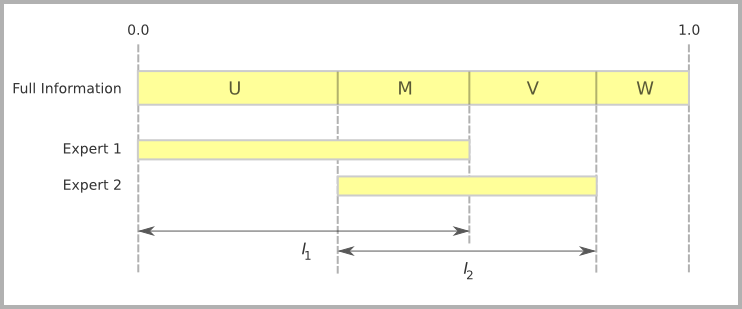
\includegraphics[width = \textwidth]{N=2} % requires the graphicx package
   \caption{Illustration of the partial information model with two experts.}
   \label{diagram2}
\end{figure}
Figure \ref{diagram2} illustrates this setup. In this diagram the Gaussian process has been partitioned into four parts based on the experts' information sets:
\begin{align*}
 U &= X_{I_1 / I_2}
& M &= X_{I_1 \cap I_2}\\
 V &= X_{I_2 / I_1}
& W &= X_{(I_1 \cup I_2)^c}
\end{align*}
Then,
\begin{align*}
X_{I_1} &= U + M\\
X_{I_2} &= M + V\\
X_S &= U+M+V+W,
\end{align*}
where $U, V, M, W$ are independent Gaussians with respective variances $\delta_1-\rho$, $\delta_2-\rho$, $\rho$, $1+\rho-\delta_1 - \delta_2$. The random variable $X_{I_j}$ can be interpreted as the information known by $E_j$. The joint distribution of $X_{S}$, $X_{I_1}$, and $X_{I_2}$ is a multivariate normal distribution. That is,
\begin{align}
\left(\begin{matrix} X_S \\ X_{I_1}\\ X_{I_2} \end{matrix}\right) &\sim \mathcal{N}\left(
 \boldsymbol{0},  \left(\begin{matrix} 
1 & \delta_1 & \delta_2\\
\delta_1 & \delta_1 &\rho\\
\delta_2 & \rho & \delta_2
 \end{matrix}\right)\right) \label{twoExperts}
\end{align}
Given that $X_S$ has mean zero, $\P(X_S > 0) = \P(A) = 0.5$. This can be viewed as the decision maker's prior probability of $A$ and is easily adjusted by changing the event $A$. More specifically, if the decision maker's prior belief is denoted with $\tilde{p}$, the event $A$ should be defined as $A = \{ X_S > \Phi^{-1}(1-\tilde{p}) \}$, where $\Phi$ represents the standard Gaussian CDF. As this paper is not concerned with any particular problem, the prior belief is taken non-informative, i.e. $\tilde{p} = 0.5$.  

\begin{figure}[htbp]
   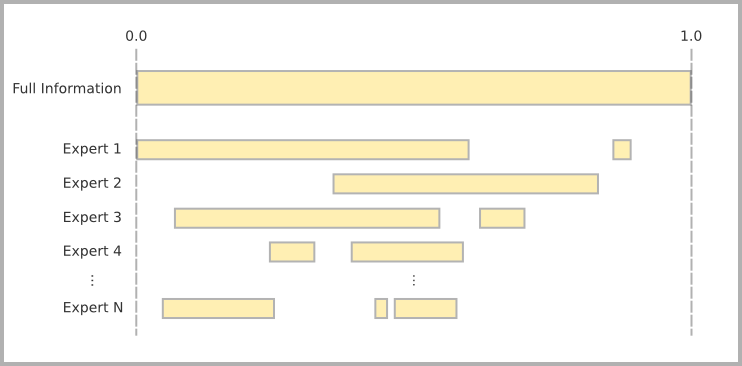
\includegraphics[width = \textwidth]{N=N} % requires the graphicx package
   \caption{Illustration of the partial information model with $N$ experts.}
   \label{diagramN}
\end{figure}



Consider now $N$ experts. Let $|I_j| = \delta_j$ be the amount of information known by expert $E_j$, and $|I_i \cap I_j| = \rho_{ij}$ be the information overlap between experts $E_i$ and $E_j$. Expression (\ref{twoExperts}) generalizes to the vector $(X_{S}, X_{I_1}, X_{I_2}, \dots, X_{I_N})$ as follows.
\begin{align}
\left(\begin{matrix} X_S \\ X_{I_1}\\ \vdots \\ X_{I_N} \end{matrix}\right) &\sim \mathcal{N}\left( \left(\begin{matrix} 
\mu_1 \\ \boldsymbol{\mu}_2
 \end{matrix}\right) =
 \boldsymbol{0}, \left(\begin{matrix} 
\Sigma_{11} & \Sigma_{12}\\
\Sigma_{21} & \Sigma_{22}\\
 \end{matrix}\right) 
 =
 \left(\begin{array}{c | c c cc }
1 & \delta_1 & \delta_2 & \dots & \delta_N  \\ \hline
\delta_1 & \delta_1 &\rho_{1,2} & \dots & \rho_{1,N}   \\ 
\delta_2 & \rho_{2,1} & \delta_2 & \dots & \rho_{2,N}  \\ 
\vdots & \vdots & \vdots & \ddots & \vdots  \\ 
\delta_N & \rho_{N,1} & \rho_{N,2} & \dots & \delta_N\\ 
 \end{array}\right)\right)  \label{NExperts}
\end{align}
This case is illustrated in Figure \ref{diagramN}. It is important to notice that $I_j$ does not have to be a contiguous segment of the unit interval. Instead, each expert can know any Borel measurable subset of the full information. Given that the information structure is described by the sub-matrix $\Sigma_{22}$, learning about the information among the $N$ experts is equivalent to estimating a covariance matrix under several restrictions. First, each element of $\Sigma_{22}$ must be in the unit interval, and no off-diagonal element can be larger than the corresponding diagonal element in the same row. Second, $\Sigma_{22}$ must be symmetric, non-singular, and coherent. The matrix $\Sigma_{22}$ is coherent if and only if its information structure can be described by a diagram such as the one given in Figure \ref{diagramN}. 


The next step is to link this model with the probability forecasts. If  $P_{I_j} = X_{I_j}/\sqrt{1-\delta_j}$ represents $E_j$'s probit-forecast, the corresponding probability forecast is given by
\begin{align}
p_j &= \P\left(A | \mathcal{F}_{I_j}\right) = \Phi\left( P_{I_j}\right) \label{Indiv}
\end{align}
This forecast is calibrated. Therefore the frequency of event occurrence agrees with the expert's assigned probabilities. For instance, consider all events that an expert believes to occur with a 60\% probability. If the expert is calibrated, 60\% of these events will actually end up occurring. Several experiments, however, have shown that experts are often poorly calibrated (see, e.g., \citet{cooke1991experts, shlyakhter1994quantifying}). Therefore assuming calibrated forecasts is hardly realistic. This could be remedied by  either including an additive error term in (\ref{Indiv}) such that each expert is on average calibrated, or by extending the total information by an amount unknown to the experts. Such an extension, however, is considered beyond the scope of this paper and hence deferred to future work. 

Recall that if $Z$ is a standard normal random variable, then $\Phi(Z)$ is uniform on $[0,1]$. Therefore the marginal distribution of $p_j$ is uniform on $[0,1]$ when the expert knows half of the information, i.e. $\delta_j = 0.5$. If the expert knows less than half of the information, i.e. $\delta_j < 0.5$, the marginal distribution of $p_j$ is unimodal at $0.5$ with the variance decreasing to 0 as $\delta_j \to 0$. Therefore an expert with no information always reports a ``non-informative" forecast of 0.5. On other hand, if the expert knows more than half of the information, i.e. $\delta_j > 0.5$, the marginal  distribution of $p_j$ is more heavily concentrated around extreme probabilities $0.0$ and $1.0$. In fact, when $\delta_j = 1$, the marginal distribution of $p_j$ is uniform over the set $\{0.0,1.0\}$. Figure \ref{marginals} illustrates the marginal distributions for $\delta_j$ equal to $0.3$, $0.5$, and $0.7$. 

\begin{figure}[t]
\centering
	\hspace{0em}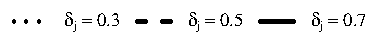
\includegraphics{LegendMarginal}

 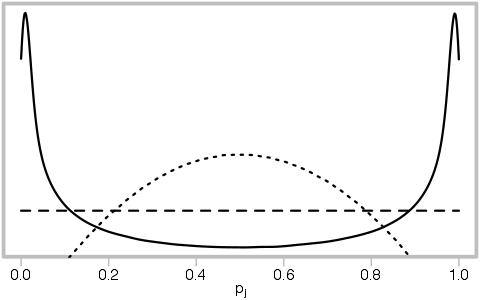
\includegraphics[width= 0.55\textwidth]{Marginals}
   \caption{The marginal distribution of $p_j$ under different levels of $\delta_j$. The more the expert knows, i.e. the higher $\delta_j$ is, the more the probability forecasts are concentrated around the extreme points 0.0 and 1.0.}
\label{marginals}
\end{figure}
%
%\subsection{Multinomial Outcomes}
%This section generalizes the partial information model to events with $K \geq 2$ outcomes. Denote these outcomes with $O_1, O_2, \dots, O_K$. Choose one of the outcomes, say $O_K$, as the base-case and define the following conditional probabilities
%\begin{align*}
%r_{jk} &= \P(O_k | O_k \cup O_K) = \frac{p_{jk}}{p_{jk}+p_{jK}},
%\end{align*}
%where $p_{jk}$ is the probability assigned to $O_k$ by the $j$th expert. Under the partial information model, these conditional probabilities are modeled similarly to the binary-case described in Section \ref{Model}. That is,
%\begin{align*}
%r_{jk} &= \Phi \left(X_{k, I_j} / \sqrt{1-\delta_{j}} \right),
%\end{align*}
%where $\{X_{k,B}\}$ is a Gaussian process defined for $O_k$. Therefore a total of $K-1$ Gaussian processes are required for an event with $K$ possible outcomes. These conditional probabilities can be mapped back to the probabilities of the individual outcomes by
%\begin{align*}
%p_{jk} &= \begin{cases}
% \frac{\frac{r_{jk}}{1-r_{jk}}}{1+\sum_{h=1}^{K-1} \frac{r_{jh}}{1-r_{jh}}} & \text{ if } k \neq K\\
% \frac{1}{1+\sum_{h=1}^{K-1} \frac{r_{jh}}{1-r_{jh}}} & \text{ if } k = K
%\end{cases}
%\end{align*}
%
%
%
%The vector of probabilities given by the $j$th expert with $\boldsymbol{p}_{j} = (p_{j1}\ p_{j2}\ \dots\ p_{j2})'$. 
%
%If the event can take upon $K \geq 2$ outcomes, one of the outcomes, say the $K$th one, is chosen as the base-case and a total of $K-1$ Gaussian processes must be constructed. The $k$th process represents the  event that the $k$th outcome occurs given that either the $k$th or the $K$th outcome occur. 
%
%This kind of behavior has been acknowledged in the previous literature (see, e.g., \cite{fox2003partition, see2006between, satopaa}).
%

%It is easy to show that all covariance matrices of size $N \times N$ are not coherent information structures. For instance, the off-diagonals of a covariance matrix  do not need to be upper bounded by its diagonal elements.  


%For instance, the matrix
%\begin{align*}
%\Sigma_{22} =  \left(\begin{array}{c c c}
%0.33 & 0.28 & 0.11\\
%0.28 & 0.33 & 0.25\\
%0.11 & 0.25 & 0.33\\
% \end{array}\right)
%\end{align*}
%is a valid covariance matrix but not a coherent information structure. The overlap $0.28$ between experts 1 and 2 is too large to allow for such a wide difference in their overlaps, $0.11$ and $0.25$ respectively, with the third expert's information set. 


%Thus $\bar{X}$ is extremized when
%\begin{align*}
% \frac{N \boldsymbol{1}_{N}' \Sigma_{22}^{-1} \boldsymbol{X}}{\boldsymbol{1}_{N}'  \boldsymbol{X}  \sqrt{N - \boldsymbol{1}_{N}' \Sigma_{22}^{-1} \boldsymbol{1}_{N}}}   &>& 1\\
% \frac{\boldsymbol{1}_{N}' \Sigma_{22}^{-1} \boldsymbol{X}}{\boldsymbol{1}_{N}'  \boldsymbol{X}  }   &>& \sqrt{ \frac{1}{N} - \frac{\boldsymbol{1}_{N}' \Sigma_{22}^{-1} \boldsymbol{1}_{N}}{N^2}},
%\end{align*}
%where the LHS side a weighed average of the elements of $\Sigma_{22}^{-1}$. This becomes clear after noticing that $\boldsymbol{X} / \boldsymbol{1}_{N}'  \boldsymbol{X}$ is a vector whose elements sum to 1. These give the weights for each respective column of $\Sigma_{22}^{-1}$. Hence the larger a given $X_j$ is the more influence it has in his weighted sum. The second term on RHS is the equally weighed average of $\Sigma_{22}^{-1}$. Notice that LHS increases as a function of $\Sigma_{22}^{-1}$ while RHS decreases. In addition, if $\boldsymbol{1}_{N}' \Sigma_{22}^{-1}  \boldsymbol{1}_{N} > \approx 1.1$ and fixed, then RHS decreases as $N$ increases. This largely revolves around understanding the interpretation of the precision matrix. 
%
%\begin{align*}
% \frac{( \boldsymbol{1}_{N}' \Sigma_{22}^{-1} \boldsymbol{X} )( \boldsymbol{X}'  \Sigma_{22}^{-1}\boldsymbol{1}_{N} )}{(\boldsymbol{1}_{N}'  \boldsymbol{X} )(  \boldsymbol{X}'  \boldsymbol{1}_{N})}   &>& \frac{1}{N} - \frac{\boldsymbol{1}_{N}' \Sigma_{22}^{-1} \boldsymbol{1}_{N}}{N^2}\\
%\end{align*}


\section{Probability Extremization}
\label{extremization}
%\textcolor{red}{Write about extremization wrt average probability}
The best in-principle forecast given the knowledge of $N$ experts is $P(X_{S} > 0 |  \mathcal{F}')$, where $\mathcal{F}' = \mathcal{F}_1 \cup \dots \cup \mathcal{F}_N$. This aggregate, however, assumes knowledge of the union of the information sets. Given that this union is almost always unattainable due to company confidentiality or the experts' inability to specify the knowledge that ultimately leads to their opinions (\cite{dawid1995coherent}), the best aggregate probability that can be realistically hoped for is  $\P(X_{S} > 0 | p_1, \dots, p_N)$. This section derives this aggregator under the partial information model and then uses it to analyze extremization.  In this paper extremization is understood as an increase in the strength of the belief indicated by the probability forecast. Therefore a probability $p$ for a binary event is extremized by $p'$ if $p'$ is closer to $0$ when $p \leq 0.5$ and closer to $1$ when $p \geq 0.5$.  

%This is generalized in the the following definition.
%\begin{definition}
%Consider a target event that can take upon $K$ outcomes. Therefore all possible probability forecasts are described with a $K$-simplex in $\mathbb{R}^{K-1}$. Let $\boldsymbol{d}$ represent the vertex of this simplex that is the closest to a $(K-1)$-dimensional probability forecast $\boldsymbol{p}$ in the simplex. This point is \textit{extremized} by another point $\boldsymbol{p}'$ in the simplex if $\boldsymbol{d}$ is closer to $\boldsymbol{p}'$ than $\boldsymbol{p}$. If, on other hand, $\boldsymbol{d}$ is closer to $\boldsymbol{p}$ than $\boldsymbol{p}'$, the forecast $\boldsymbol{p}$ is \textit{reverse-extremized} by $\boldsymbol{p}'$.
%\end{definition}

To derive the partial information aggregator, let $\boldsymbol{X}$ be a column vector of length $N$ such that $X_j = X_{I_j}$ for $j = 1, \dots, N$. If $\Sigma_{22}$ is a coherent overlap structure and $\Sigma_{22}^{-1}$ exists, then $X_{S} | \boldsymbol{X} \sim \mathcal{N}(\bar{\mu}, \bar{\Sigma})$, where
\begin{align}
\bar{\mu} &= \mu_1 + \Sigma_{12} \Sigma_{22}^{-1} (\boldsymbol{X} - \boldsymbol{\mu}_2) =  \Sigma_{12} \Sigma_{22}^{-1} \boldsymbol{X} \label{condMu}
\end{align}
and
\begin{align}
 \bar{\Sigma}&= \Sigma_{11} - \Sigma_{12} \Sigma_{22}^{-1} \Sigma_{21} =1 - \Sigma_{12} \Sigma_{22}^{-1} \Sigma_{21}  \label{condSigma}
\end{align}
These expression can be derived directly from the formulas of the conditional multivariate Gaussian distribution (see, e.g., Result 5.2.10 on p. 156 in \cite{ravishanker2001first}). The result is the following class of probability aggregators indexed by $\Sigma_{22}$.
\begin{align}
\P\left(A  | \boldsymbol{X}\right)  = \P\left(X_{S} > 0 | \boldsymbol{X}\right) &= \Phi\left( \frac{\Sigma_{12} \Sigma_{22}^{-1} \boldsymbol{X}}{\sqrt{1 - \Sigma_{12} \Sigma_{22}^{-1} \Sigma_{21}}}\right) \label{GeneralAggregator}
%&= \Phi\left( \frac{\boldsymbol{1}_{N}'  \Sigma_{22}^{-1} \Phi^{-1}(\boldsymbol{p})}{\sqrt{1 - \boldsymbol{1}_{N}' \Sigma_{22}^{-1} \boldsymbol{1}_{N}}}\right)
\end{align}
%This aggregator and the distribution of $\boldsymbol{p} = (p_1, p_2, \dots, p_N)$, as is induced by (\ref{NExperts}), form a consistent pair 

To link this with extermination, collect all probit-forecasts into a vector $\boldsymbol{P} = (P_{I_1} P_{I_2} \dots P_{I_N})'$, denote the average probit-forecast with $\bar{P} = \left( \sum_{j=1}^N P_{I_j} \right)/N$, and use $\alpha$ to represent the amount of extremization that the partial information aggregator (\ref{GeneralAggregator}) performs for $\bar{P}$. Then,
\begin{align}
\alpha \bar{P}&=  \frac{\Sigma_{12} \Sigma_{22}^{-1} \boldsymbol{X}}{\sqrt{1 - \Sigma_{12} \Sigma_{22}^{-1} \Sigma_{21}}}  &\Leftrightarrow&& \alpha  = \frac{N \Sigma_{12} \Sigma_{22}^{-1} \boldsymbol{X}}{\left(\boldsymbol{1}_N' \boldsymbol{P} \right) \sqrt{1 - \Sigma_{12} \Sigma_{22}^{-1} \Sigma_{21}}} \label{alpha}
\end{align}
The partial information aggregate extremizes $\bar{P}$ when $\alpha$ is greater than $1$. In the contrary, when $\alpha$ is less than 1, the partial information aggregate reverse-extremizes $\bar{P}$. Even though this paper focuses on extremization of the average probit forecast, the discussion can be easily applied to the average logit-forecast by recalling that $\text{logit}(p_i) \approx \Phi^{-1}(p_i)/\sqrt{\frac{\pi}{8}}$. Therefore the amount of extremization that the partial information aggregator performs for the average logit-forecast is $\sqrt{\frac{\pi}{8}} \approx 0.627$ times $\alpha$.  


As the extremizing factor $\alpha$ is not necessarily greater or equal to 1, the partial information aggregator (\ref{GeneralAggregator}) does not always yield an extremized probability. A case-by-case analysis reveals that the aggregator extremizes most of the time. Therefore it seems more prudent to focus the discussion on cases that do not lead to extremization. The following two examples illustrate two main sources of reverse-extremization. For the sake of clarity, the examples involve only two experts. 

%\textcolor{red}{EXPLAIN THAT THE AGGREGATE IS OFTEN MORE EXTREME THAN THE GROUP OR AT LEAST CAN BE OUTSIDE. CITE PAGES SECOND PAPER.}


\begin{example}
\label{Example1}
\textbf{Dominating Expert.} This example illustrates that the amount of extremization can be driven by an expert whose information forms a superset of information. To make this more concrete, consider the following setup.
\begin{align*}
\Sigma_{22} =  \left(\begin{array}{c c}
0.20 & 0.20\\
0.20 & 0.40 \\
 \end{array}\right)
  && 
  \begin{array}{l l}
X_{I_1} =& -0.80\\
X_{I_2} =& 0.30
 \end{array}
\end{align*}
The probability forecasts in this example are $p_1 = 0.19$ and $p_2 = 0.65$, the average probability is $\bar{p} = 0.42$, and the average probit forecast (transformed to probability space) is $\Phi(\bar{P}) = 0.40$. 
The partial information aggregate is $0.65$.  Given that this is more than 0.5 while $\bar{p}$ and $\Phi(\bar{P})$ are less than 0.5, the extremizing constant is negative. To understand this result, notice that expert $E_2$ knows everything that expert $E_1$ knows. Therefore $E_1$ does not provide any new information and can be ignored. The partial information aggregate is exactly the same as the probability forecast made by $E_2$. Given that only the partial information aggregator is able to take into account overlap information, its aggregate can differ radically from the average probability and probit-forecast when the experts share information.
\end{example}

By varying the overlap coefficient $\rho$ in Example \ref{Example1}, it is possible to establish any qualitative relationship between the partial information aggregate and the other two aggregators. Therefore no single extremization rule can always hold, and inferring the information distribution among the experts is highly important. Estimating the information structure, however, is not in the scope of this paper and is hence left for future work. Before describing the second source of reverse-extremization, it is helpful to introduce the class of non-overlapping information structures. 

\subsection{Non-overlapping Information}
\label{nonoverlap}
This section assumes that the experts' information sets do not overlap, i.e.   $|I_{i} \cap I_{j}| = \emptyset$ for all $i \neq j$. The resulting information structure is diagonal.  That is,
% $\rho \in [\max \{(N-T)/(T(N-1)), 0\},1] = A_\rho$. 
\begin{align*}
\left(\begin{matrix} X_{S} \\ X_{I_1}\\ \vdots \\ X_{I_N} \end{matrix}\right) &\sim \mathcal{N}\left( 
 \boldsymbol{0}, \left(\begin{matrix} 
\Sigma_{11}^{(no)} & \Sigma_{12}^{(no)}\\
\Sigma_{21}^{(no)} & \Sigma_{22}^{(no)}\\
 \end{matrix}\right) 
 =
 \left(\begin{array}{c|cccc}
1 & \delta_1 & \delta_2 & \dots & \delta_N  \\ \hline
\delta_1 & \delta_1 &0 & \dots & 0   \\ 
\delta_2 & 0 & \delta_2 & \dots & 0  \\ 
\vdots & \vdots & \vdots & \ddots & \vdots  \\ 
\delta_N & 0 & 0 & \dots & \delta_N\\ 
 \end{array}\right)\right),
\end{align*}
where the super-script $(no)$ emphasizes that this information structure is non-overlapping and hence different from the fully general structure described in (\ref{NExperts}). The information structure $\Sigma_{22}^{(no)}$  is coherent if and only if $\sum_{j=1}^N \delta_j \leq 1$ with all $\delta_j \in [0,1]$. The resulting aggregator is 
\begin{align}
\P\left(X_{S} > 0 | \boldsymbol{X}\right) &= \Phi\left( \frac{\sum_{j=1}^N X_{I_j}}{\sqrt{1 - \sum_{j=1}^N \delta_j}}\right) \label{VotingAggre}
\end{align}
This aggregator can be described in two steps: The first step is voting where votes are weighted according to the importance of the experts' private information. This step is performed by the summation in the numerator. If this sum falls below $0.0$ (or above $0.0$), the consensus believes that the event will not happen (or will happen). The second step is performed by the denominator that extremizes the experts' belief according to the total amount of information in the group. For instance, if the experts know all the information, i.e. $\sum_{j=1}^N \delta_j = 1$, their vote deterministically indicates whether the event $A$ happens or not. These steps do not necessarily lead to extremization. This shown in the next example that discusses the second source of reverse-extremization.

\begin{example}
\label{KeyInfo}
\textbf{Highly Influential Information.} This example illustrates that the amount of extremization can be driven by a highly influential piece of information. To make this more specific, consider the following setup.
\begin{align*}
\Sigma_{22} =  \left(\begin{array}{c c}
0.05 & 0.00\\
0.00 & 0.90 \\
 \end{array}\right)
  && 
  \begin{array}{l l}
X_{I_1} =& 0.50\\
X_{I_2} =& -0.25
 \end{array}
\end{align*}
The probability forecasts in this example are $p_1 = 0.70$ and $p_2 = 0.21$, the average probability is $\bar{p} = 0.46$, and the average probit forecast (transformed to probability space) is $\Phi(\bar{P}) = 0.44$.  The partial information aggregate is $0.87$. Therefore the extremizing constant is negative. As the information structure is diagonal, the partial information aggregate resembles voting that gives each $X_{I_j}$ equal weight despite how much the corresponding expert knows. The consensus is that the event will happen. Given that the experts know 95\% of the information, their consensus belief is extremized heavily leading to a final aggregate of $0.87$. The other two aggregates fall below $0.5$ because they weight $E_2$'s information much more than $E_1$'s information.
\end{example}

Example \ref{KeyInfo} illustrates that the partial information aggregate can be outside the convex hull of the experts' probability forecasts. This is a desirable in aggregation of beliefs that have been derived from attributes associated with the target event (see \cite{parunak2013characterizing} for a detailed discussion). Given that the non-overlapping information structure excludes the possibility of a dominating expert, aggregator (\ref{VotingAggre}) can be expected to extremize in the absence of highly influential information. 
% It is possible to show that the aggregator (\ref{VotingAggre}) always extremizes the probit forecast when each $X_{I_j}$ falls on the same side of zero; that is, when there is no highly influential piece of information. 
% 
One version of this statement is given in the following observation.
 
\begin{observation}
\label{positiveThmVote}
Under the non-overlapping information structure, the extremizing factor, $\alpha$, is greater or equal to $1$ if either $X_{I_j} \geq 0$ or  $X_{I_j} \leq 0$, or equivalently $p_j \geq 0.5$ or $p_j \leq 0.5$ simultaneously for all $j = 1, \dots, N$. 
\end{observation}
\begin{proof} 
Let $\boldsymbol{d} = \frac{1}{N}\left((1-\delta_1)^{-1/2}, (1-\delta_2)^{-1/2}, \dots, (1-\delta_N)^{-1/2}\right)'$. Assume without loss of generality that $\bar{P} > 0$. Then the average probit forecast is extremized if
\begin{align}
 \bar{P}&\leq  \frac{\sum_{j=1}^N X_{I_j}}{\sqrt{1 - \sum_{j=1}^N \delta_j}} &\Leftrightarrow&& 0 \leq  \left(  \left(1 - \sum_{j=1}^N \delta_j \right)^{-1/2} \boldsymbol{1}_N - \boldsymbol{d}' \right) \boldsymbol{X} \label{votingproof}
\end{align}
 As $N (1-\delta_j)^{1/2} \geq \left(1 - \sum_{j=1}^N \delta_j \right)^{1/2}$ for all $j = 1, \dots, N$, all the elements of $$\left(1 - \sum_{j=1}^N \delta_j \right)^{-1/2} \boldsymbol{1}_N - \boldsymbol{d}' $$ are non-negative. Therefore the right hand side of (\ref{votingproof}) is always non-negative. 
\end{proof}
The next section discusses a class of information structures that is unaffected by both sources of reverse-extremization. The result is an aggregator that always extremizes the average probit-forecast. 

\subsection{Compound Symmetric Information}
\label{compound}

This section assumes that the experts' information sets have the same size and that the amount of overlap between any two information sets is constant, i.e.  $|I_{1}| =  \dots = |I_{N}|$ and $|I_{i} \cap I_{j}| = |I_{h} \cap I_{k}|$ for all $i \neq j$ and $h \neq k$. In other words, each expert knows and shares the same amount with every other expert. Therefore the experts are exchangeable, and no single expert can dominate. The resulting information structure is compound symmetric. That is,
% $\rho \in [\max \{(N-T)/(T(N-1)), 0\},1] = A_\rho$. 
\begin{align*}
\left(\begin{matrix} X_{S} \\ X_{I_1}\\ \vdots \\ X_{I_N} \end{matrix}\right) &\sim \mathcal{N}\left( 
 \boldsymbol{0}, \left(\begin{matrix} 
\Sigma_{11}^{(cs)} & \Sigma_{12}^{(cs)}\\
\Sigma_{21}^{(cs)} & \Sigma_{22}^{(cs)}\\
 \end{matrix}\right) 
 =
 \left(\begin{array}{c|cccc}
1 & \delta & \delta & \dots & \delta  \\ \hline
\delta & \delta &\rho\delta & \dots & \rho\delta   \\ 
\delta & \rho\delta & \delta & \dots & \rho\delta  \\ 
\vdots & \vdots & \vdots & \ddots & \vdots  \\ 
\delta & \rho\delta & \rho\delta & \dots & \delta\\ 
 \end{array}\right)\right),
\end{align*}
where the super-script $(cs)$ emphasizes that this information structure is compound symmetric and hence different from the fully general structure described in (\ref{NExperts}). The amount known by each expert is denoted with $\delta \in [0,1]$. The shared proportion of the known information is 
\begin{align}
\rho &\in \left[  \max \left\{ \frac{N-\delta^{-1}}{N-1}, 0\right\}, 1 \right] \label{rhoDomain}
\end{align}
The positive lower bound for $\rho$ is necessary because overlap in the information sets becomes unavoidable when $\delta > 1/N$. To compute the lower bound, assume $\delta > 1/N$ and let $I_{i} \cap I_j = I$ and $|I| =  \rho \delta$ for all $i \neq j$. The minimum sharing occurs when all information is either public or private; that is, when $\rho\delta + N(\delta - \delta\rho) = 1$. This equality gives the desired lower bound. The quantity  $\rho\delta + N(\delta - \delta\rho)$ also describes the maximum information coverage of the $N$ experts, i.e. $\max | I_1 \cup I_2 \cup \dots \cup I_N| = \rho\delta + N(\delta - \delta\rho)$. 

In practice the values of $\delta$ and $\rho$ can be estimated via the maximum likelihood method. To make this more explicit, observe that $\boldsymbol{P} \sim \mathcal{N}_N\left(\boldsymbol{0}, \Sigma_{22}^{(cs)} (1-\delta)^{-1}\right)$ and that the Jacobian for the map $\boldsymbol{P} \to \Phi\left(\boldsymbol{P}\right)$ is
\begin{eqnarray*}
J(\boldsymbol{X}) &=& (2\pi)^{-N/2} \exp \left( - \frac{\boldsymbol{P}' \boldsymbol{P}}{2}   \right) 
\end{eqnarray*}
If $h(\boldsymbol{P})$ denotes the multivariate Gaussian density of $\boldsymbol{P}$,  
%by the Inverse Function Theorem 
the density for  $\boldsymbol{p} = (p_1, p_2, \dots, p_N)$ is 
\begin{eqnarray*}
 f\left(p_1, \dots, p_N | \delta, \rho \right) &=& h(\boldsymbol{P}) J(\boldsymbol{P})^{-1} \bigg|_{\boldsymbol{P} = \Phi^{-1}(\boldsymbol{p})}\\
%&=& \frac{(1-\delta)^{N/2}}{\sqrt{ |\Sigma_{22}|}} \exp\left( -\frac{1}{2} \boldsymbol{P}' (1-\delta)\Sigma_{22}^{-1} \boldsymbol{P} + \frac{\boldsymbol{P}' \boldsymbol{P}}{2}   \right)\\
&=& \frac{(1-\delta)^{N/2}}{\sqrt{ |\Sigma_{22}^{(cs)}|}} \exp\left( -\frac{1}{2} \Phi^{-1}(\boldsymbol{p})' \left( (1-\delta) \left(\Sigma_{22}^{(cs)}\right)^{-1} - I_N \right) \Phi^{-1}(\boldsymbol{p})  \right) 
\end{eqnarray*}
where $\Phi^{-1}(\boldsymbol{p}) =  (\Phi^{-1}(p_1), \Phi^{-1}(p_2), \dots, \Phi^{-1}(p_N))$. 
%Given that $\Sigma_{22}^{(cs)}$ can be written in the form  $\Sigma_{22}^{(cs)} = I_N (\delta-\rho\delta) + J_{N \times N} \rho\delta$
The inverse of $\Sigma_{22}^{(cs)}$  is
\begin{align}
\left(\Sigma_{22}^{(cs)}\right)^{-1} = I_N \left(\frac{1}{\delta-\rho\delta} \right) - J_{N \times N} \frac{\rho}{(1-\rho)\delta(1+(N-1) \rho)} \label{inverse},
\end{align}
where $J_{N \times N}$ is a matrix of ones with $N$ columns and rows (see the supplementary material of \cite{dobbin2005sample} for the proof of this fact).  According to p. 32 in \cite{rao2009linear}, the determinant of $\Sigma_{22}^{(cs)}$ is
\begin{align*}
%| \Sigma_{22}| = (\delta - \rho\delta)^N \left(1+\frac{N \delta \rho}{\delta - \delta\rho} \right),
\left| \Sigma_{22}^{(cs)}\right| = (\delta(1- \rho))^N \left(1+\frac{N \rho}{1 - \rho} \right),
\end{align*}
The maximum likelihood estimates of $\delta$ and $\rho$ are then obtained from
\begin{align}
(\hat{\delta}, \hat{\rho}) =& \argmax_{\rho, \delta} \log  f\left(p_1, \dots, p_N | \delta, \rho \right), \label{MLE}\\
& \text{s.t. } \nonumber \delta \in [0,1] \text{ and } \rho \in \left[  \max \left\{ \frac{N-\delta^{-1}}{N-1}, 0\right\}, 1 \right]
\end{align}
Unfortunately, (\ref{MLE}) cannot be solved analytically. However, a simple grid-search can be used to find the estimates very efficiently. 

%\begin{align*}
%(\hat{\delta}, \hat{\rho}) &= \argmax_{\rho, \delta}  - \frac{N}{2} \log (\delta - \rho\delta) - \frac{1}{2} \log \left(1+\frac{N \delta \rho}{\delta - \delta\rho} \right) -\frac{1}{2} \boldsymbol{X}' \left( I_N \left(\frac{1}{\delta-\rho\delta} \right) - J_{N \times N} \frac{\rho}{(1-\rho)\delta(1+(N-1) \rho)}  \right) \boldsymbol{X}
%\end{align*}




%Recall that if $X_{I_j} \sim \mathcal{N}(0,1)$, then $\Phi(X_{I_j})$ is uniform on $[0,1]$. Therefore, if $\delta_j = 1$, the marginal distribution of $p_j = \Phi(X_{I_j})$ is uniform on $[0,1]$. If this does not hold empirically, it is a sign that the model cannot be correct on the micro-level. If $X_{I_j}$ appears more (respectively less) concentrated about $0.5$, then the model can be adjusted by changing $\delta_{j}$ to a smaller fraction. 


%Assuming no further prior information on overlap structure, the expected amount of information held by the group is WHAT IS THIS?

The aggregator under the compound symmetric information structure can be derived by applying (\ref{inverse}) to the general formulas (\ref{condMu}) and (\ref{condSigma}). The resulting conditional mean and variance are 
%By the conditional multivariate normal results, we have that 
%\begin{align*}
%\bar{\mu} &= \mu_1 + \Sigma_{12} \Sigma_{22}^{-1} (\boldsymbol{X} - \boldsymbol{\mu}_2)\\
% &= \Sigma_{12} \Sigma_{22}^{-1} \boldsymbol{X} \\
% \\
% \bar{\Sigma}&= \Sigma_{11} - \Sigma_{12} \Sigma_{22}^{-1} \Sigma_{21}\\
%&=1 - \Sigma_{12} \Sigma_{22}^{-1} \Sigma_{21}
%\end{align*}
%
%%(see \url{http://linus.nci.nih.gov/techreport/DobbinSimonAppendix.pdf} for this). 
%Hence the off-diagonals of $\Sigma_{22}^{-1}$ are 
%\begin{align*}
%\frac{\rho\delta}{(\rho\delta-\delta)((N-1)\rho\delta +\delta)}
%\end{align*}
%and the diagonals are
%\begin{align*}
%\frac{(2-N)\rho\delta -\delta}{(\rho\delta-\delta)((N-1)\rho\delta +\delta)}
%\end{align*}
%The conditional mean can be derived as
%\begin{align*}
%\Sigma_{22}^{-1} &= \frac{1}{(\rho\delta-\delta)((N-1)\rho\delta +\delta)}
% \left(\begin{matrix} 
%(2-N)\rho\delta -\delta & \rho\delta & \dots & \rho\delta \\ 
%\rho\delta & (2-N)\rho\delta -\delta & \dots & \rho\delta \\ 
%\vdots & \vdots &  \ddots & \vdots \\ 
%\rho\delta & \rho\delta & \dots & (2-N)\rho\delta -\delta  \\ 
% \end{matrix}\right)\\
% \Sigma_{12} \Sigma_{22}^{-1} &= \frac{\delta}{(\rho\delta-\delta)((N-1)\rho\delta +\delta)} \left( \begin{matrix} \rho\delta -\delta &  \dots & \rho\delta -\delta \end{matrix} \right)\\
% \Sigma_{12} \Sigma_{22}^{-1} \boldsymbol{X} &= \frac{\delta}{(\rho\delta-\delta)((N-1)\rho\delta +\delta)} (\rho\delta -\delta) \sum_{j=1}^N X_j \\
%&= \frac{\delta(\rho\delta -\delta)}{(\rho\delta-\delta)((N-1)\rho\delta +\delta)}  \sum_{j=1}^N X_j \\
%&= \frac{\delta}{(N-1)\rho\delta +\delta}  \sum_{j=1}^N X_j \\
\begin{align*}
\bar{\mu} = \frac{1}{(N-1)\rho +1}  \sum_{j=1}^N X_j 
% \bar{\Sigma} &= 1 -  \Sigma_{12} \Sigma_{22}^{-1}\Sigma_{21} \\
% &= 1  - \frac{\delta^2}{(\rho\delta-\delta)((N-1)\rho\delta +\delta)} N(\rho\delta -\delta)\\
% &= 1  - \frac{\delta^2N}{(N-1)\rho\delta +\delta} \\
&&  \bar{\Sigma} = 1  - \frac{\delta N}{(N-1)\rho +1} 
\end{align*}
Therefore the  aggregator becomes
\begin{align}
\P\left(X_S > 0 | \boldsymbol{X}\right) &=\Phi\left(\frac{\frac{1}{(N-1)\rho +1} \sum_{j=1}^N X_{I_j} }{\sqrt{1- \frac{N\delta}{(N-1)\rho +1} }}  \right) \label{CompoundAggre}
\end{align}
%It is crucial to notice that this aggregator can learn the amount of extremization without a separate training set. Therefore it can be applied to a wide range of applied problems. 
Equating this with $\alpha \bar{P}$ results in the following extremizing factor.
\begin{align}
%\alpha \bar{X}  &=  \frac{\frac{1}{(N-1)\rho +1} \sum_{j=1}^N X_j }{\sqrt{T- \frac{N}{(N-1)\rho +1} }}\\
%\alpha &= \frac{\frac{1}{(N-1)\rho +1} \sum_{j=1}^N X_j }{\bar{X} \sqrt{T- \frac{N}{(N-1)\rho +1} }}\\
\alpha &= \frac{\frac{N\sqrt{1-\delta}}{(N-1)\rho +1}}{\sqrt{1- \frac{N\delta}{(N-1)\rho +1} }} \label{CompoundAlpha}
% &= \frac{\frac{N}{(N-1)\rho +1}}{\sqrt{1-\delta  \left( \frac{N}{(N-1)\rho +1}  \right)}} \\
% &= \frac{\gamma}{\sqrt{1-\delta\gamma}},
% &= \frac{N}{\sqrt{((N-1)\rho +1)^2 (T- \frac{N}{(N-1)\rho +1} )}}\\
% &= \frac{N}{\sqrt{((N-1)\rho +1)^2T- N((N-1)\rho +1) )}}
\end{align}
%where 
%\begin{align*}
%\gamma &= \frac{N}{(N-1)\rho +1}\\
%&= \left( \frac{1}{(N-1)\rho +1} \right) N\\
%\end{align*}
%WHAT IS GAMMA? Given that 
%\begin{align*}
%\gamma \delta &\leq 1\\
%% \frac{N \delta}{(N-1)\rho +1}  &\leq& 1\\
% \frac{N\delta - 1}{N-1}  &\leq \rho,
%\end{align*}
Given that the square-root is not defined for negative values,  it must be required that
\begin{align}
1- \frac{N\delta}{(N-1)\rho +1}  &\geq 0 &\Leftrightarrow&& \rho \geq \frac{N\delta - 1}{N-1} \label{rhoDomain2}
\end{align}
Contrast this with former domain restriction (\ref{rhoDomain}) and observe that both $N\delta - 1$ and $N - \delta^{-1}$ are negative when $\delta < 1/N$. Given that $N\delta - 1 > N - \delta^{-1}$ only when $\delta < 1/N$, the latter domain restriction (\ref{rhoDomain2}) is redundant and can be ignored. 

Expression (\ref{CompoundAlpha}) is positively associated with $N$ and $\delta$ but negatively associated with $\rho$. Therefore the amount of extremization is positively associated with the total amount of information in the group of expert. As expression (\ref{CompoundAlpha}) does not depend on $\boldsymbol{X}$, the amount of extremization cannot be driven by highly influential information. Therefore, given that the amount of extremization is unaffected by both sources of reverse-extremization, it is not surprising that the aggregator (\ref{CompoundAggre}) always extremizes. This is stated more formally in the following observation.

\begin{observation}
\label{positiveThm}
Under the compound symmetric information structure, the extremizing factor $\alpha$ is always greater or equal to 1. 
\end{observation}
\begin{proof} 
For a given $\delta$, the extremizing constant $\alpha$ is minimized when $(N-1)\rho +1$ is maximized. This happens at $\rho = 1$. Plugging this into (\ref{CompoundAlpha}) gives
\begin{align*}
\alpha &= \frac{\frac{N\sqrt{1-\delta}}{(N-1)\rho +1}}{\sqrt{1- \frac{N\delta}{(N-1)\rho +1} }}  \geq \frac{\sqrt{1-\delta}}{\sqrt{1-\delta }} = 1
\end{align*}
\end{proof}




%As $\frac{N}{(N-1)\rho +1} \in [1, N]$, this quantity can be thought of as the amount of knowledge that the group knows. Therefore $\alpha$ is a ratio of the amount of knowledge known and the amount of knowledge that is unknown to the group. This makes intuitively sense because if the group knows almost all of $T$, then their average should be heavily extremized.
% If the group of experts is large, then $N-1 \approx N$ and 
%\begin{align*}
%\alpha &= \frac{\frac{N}{N\rho +1} }{\sqrt{T- \frac{N}{N\rho +1} }}
%\end{align*}
%
%
%
%\begin{figure}[hbt!]
%\begin{minipage}[t]{0.33\textwidth}
%\centering
%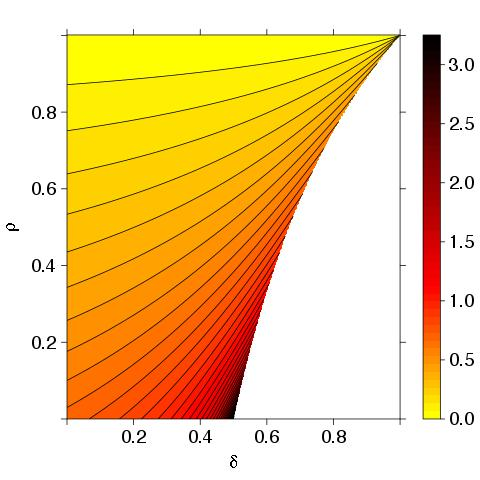
\includegraphics[width=\textwidth, height = \textwidth]{ExtremeN2.jpeg}
%\caption{N = 2}
%\label{ExtremeN5}
%\end{minipage}
%\begin{minipage}[t]{0.33\textwidth}
%\centering
%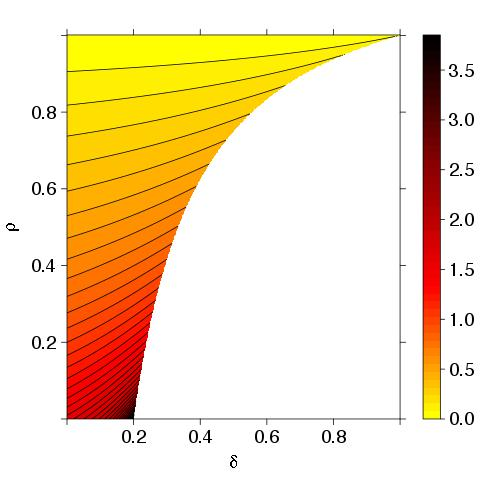
\includegraphics[width=\textwidth, height = \textwidth]{ExtremeN5.jpeg}
%\caption{N = 5}
%\label{ExtremeN10}
%\end{minipage}
%\begin{minipage}[t]{0.33\textwidth}
%\centering
%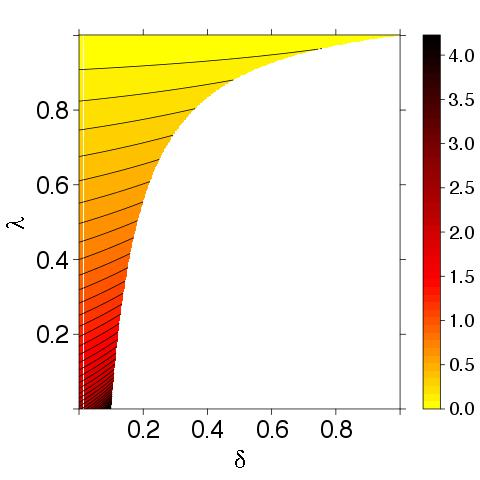
\includegraphics[width=\textwidth, height = \textwidth]{ExtremeN10.jpeg}
%\caption{N = 10}
%\label{ExtremeN30}
%\end{minipage}
%\end{figure}


\begin{figure}
        \centering
        \begin{subfigure}[b]{0.45\textwidth}
                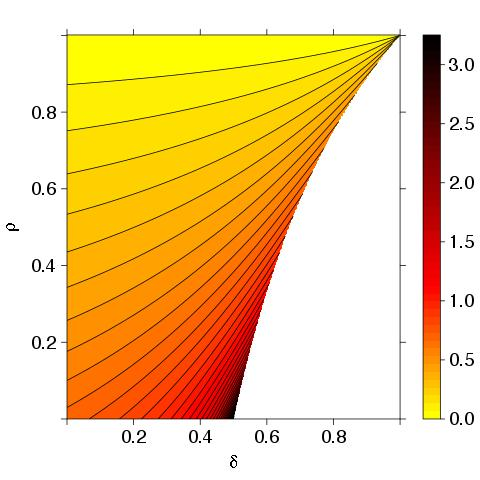
\includegraphics[width=\textwidth]{ExtremeN2.jpeg}
\caption{N = 2}	
\label{ExtremeN5}
        \end{subfigure}%
        ~ %add desired spacing between images, e. g. ~, \quad, \qquad etc.
          %(or a blank line to force the subfigure onto a new line)
%        \begin{subfigure}[b]{0.32\textwidth}
%                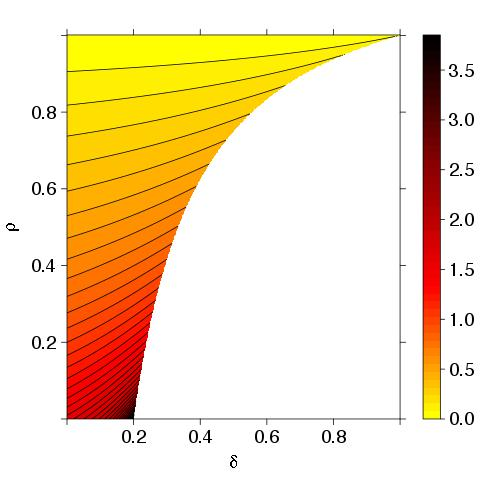
\includegraphics[width=\textwidth]{ExtremeN5.jpeg}
%\caption{N = 5}
%\label{ExtremeN10}
%        \end{subfigure}
        ~ %add desired spacing between images, e. g. ~, \quad, \qquad etc.
          %(or a blank line to force the subfigure onto a new line)
        \begin{subfigure}[b]{0.45\textwidth}
                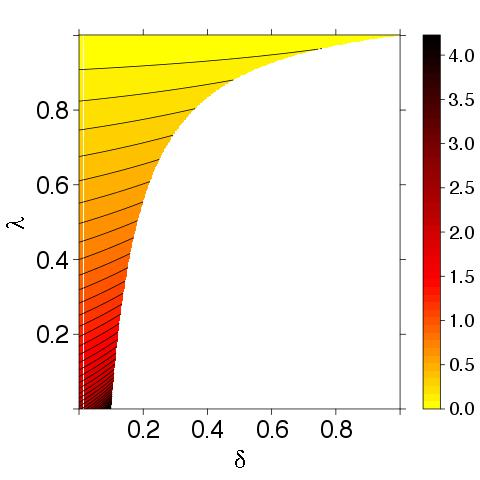
\includegraphics[width=\textwidth]{ExtremeN10.jpeg}
\caption{N = 10}
\label{ExtremeN30}
        \end{subfigure}
        \caption{ The amount of log-extremization $\log(\alpha)$ under different combinations of $N$ (the number of experts), $\delta$ (the amount of information known by one expert), and $\rho$ (the amount of information shared by any two experts).}
\end{figure}



Because the extremizing factor (\ref{CompoundAlpha}) depends only on three intuitive parameters, it can be analyzed graphically. Figures \ref{ExtremeN5} and \ref{ExtremeN30} describe the amount of log-extremization $\log(\alpha)$ under different values of $\rho, \delta$, and $N$. High values have been censored to keep the scale manageable. By Observation \ref{positiveThm} the amount of extremizing is always greater or equal to 1.0. The extremizing factor increases indefinitely towards the point $\delta = 1/N$ and $\rho = 0$. In this case the experts' information sets form a partition of the full information. Therefore the experts know all the information. Such a group of experts can re-construct $X_S$ by simply adding up their  information. This turns aggregation into deterministic voting: if the sum of the probit-forecasts is above 0, the event $A$ materializes; else it does not. A similar observation has been made by  \cite{hong2009interpreted}. 

 

%Moving towards the upper left corner, where $\delta = 0.0$ and $\rho = 1.0$, decreases the amount of extremizing monotonically to $1.0$.
The amount of extremization decreases as a) the amount of information that each individual expert holds decreases and/or b) the amount of shared information increases. Therefore the more knowledgable and diverse the group of experts is, the more their average probit-forecast should be extremized. This observation aligns with the earlier discussion in Section \ref{nonoverlap}. The only exception occurs when $\rho = 1.0$. In this case, all information is public, and the group of experts is as good as a single expert. Therefore, given that a single expert's forecast should not be extremized, $\rho = 1.0$ always implies $\alpha = 1.0$ regardless of the value of $\delta$. 


From Figures \ref{ExtremeN5} and \ref{ExtremeN30} it is clear that the feasible set of $(\delta, \rho)$-values becomes smaller as $N$ increases. This limitation arises from assuming a compound symmetric overlap structure. Having many experts, each with a considerable amount of information, simply leads to unavoidable overlap in the information sets. From the domain restriction (\ref{rhoDomain}), it is clear that $\rho \to 1$ as $N \to \infty$. Therefore in the limit the group of experts is equivalent to a single expert. This observation clearly does not reflect the real-world. When $N = 2$, on other hand, the compound symmetric overlap is almost fully general. Therefore assuming a compound symmetric information structure can be appropriate for small numbers of experts but becomes overly restrictive as more experts enter the group. 

%\subsection{Information in the Sample Average}
%It is possible to determine the amount of information in the sample average. This is done by first computing the aggregate probability for the sample average, and then finding the amount of information that a single expert should have in order for his aggregate probability to match with the aggregate probability of the sample average. That is, if $\delta_X$ denotes the information in the sample average, then 
%\begin{align*}
%%\frac{1}{\sqrt{1-\delta_X}} &= \frac{\frac{N}{(N-1)\rho +1}}{\sqrt{1- \frac{N\delta}{(N-1)\rho +1} }} \\
%\alpha &= \frac{1}{\sqrt{1-\delta_X}} &\Leftrightarrow&& \delta_X &=1-\alpha^{-2}
%\end{align*}
%Based on these equation we notice that there is a monotonic and positive relationship between $\alpha$ and $\delta_X$. This means that the more the sample average is extremized the more information it contains, and \textit{vice versa}. This result is interesting because it allows the researcher to first use black-box models from earlier literature to determine the amount of extremization and then use this quantity to analyze the portion of information that is present in the sample average. 

%
%
%\subsection{Integrate over the prior distribution}
%
%In this section we assumed that we know how much each expert knows but have no idea how much each information each experts shares. Denote $M = \max \left\{ \frac{N\delta-1}{N-1}, 0\right\}$ and assume a uniform prior on $\rho \in [M, \delta]$. That is, let $p(\rho) = (\delta - M)^{-1}$. Then,
%\begin{align*}
%\E_\rho[\alpha] &= \E \left[\frac{\frac{\delta N}{(N-1)\rho +\delta}}{\sqrt{1- \frac{N\delta^2}{(N-1)\rho +\delta} }} \right]\\
%&= (\delta - M)^{-1}  \int_{M}^\delta \frac{\frac{\delta N}{(N-1)\rho +\delta}}{\sqrt{1- \frac{N\delta^2}{(N-1)\rho +\delta} }}   d\rho\\
%\end{align*}
%Let $z = (N-1)\rho +\delta$. Then $dz = (N-1)d\rho \Rightarrow (N-1)^{-1}dz = d\rho$   and 
%\begin{align*}
%&= \frac{1}{(N-1)(\delta - M)}  \int_{(N-1)M+\delta}^{N\delta} \frac{\frac{\delta N}{z} }{\sqrt{1- \frac{N\delta^2}{z} }}  dz\\
%&= \frac{N\delta}{(N-1)(\delta - M)} \int_{(N-1)M+\delta}^{N\delta} \frac{1}{\sqrt{z^2- N\delta^2 z }}  dz\\
%&= \frac{N\delta}{(N-1)(\delta - M)} \int_{(N-1)M+\delta}^{N\delta} \frac{1}{\sqrt{z^2- 2 \frac{N\delta^2}{2} z + \left( \frac{N\delta^2}{2} \right)^2 - \left( \frac{N\delta^2}{2} \right)^2}}  dz\\
%&= \frac{N\delta}{(N-1)(\delta - M)} \int_{(N-1)M+\delta}^{N\delta} \frac{1}{\sqrt{\left( z- \frac{N\delta^2}{2} \right)^2 - \left( \frac{N\delta^2}{2} \right)^2}}  dz
%\end{align*}
%Let $u =  z- \frac{N\delta^2}{2}$. Then $du = dz$ and 
%\begin{align*}
%&=\frac{N\delta}{(N-1)(\delta - M)} \int_{(N-1)M+\delta- \frac{N\delta^2}{2}}^{N\delta- \frac{N\delta^2}{2}} \frac{1}{\sqrt{u^2 - \left( \frac{N\delta^2}{2} \right)^2}}  du\\
%&= \frac{N\delta}{(N-1)(\delta - M)} \left\{\log \left(\sqrt{4u^2 - \delta^4N^2} + 2u \right) \right\}\bigg|_{(N-1)M+\delta- \frac{N\delta^2}{2}}^{N\delta- \frac{N\delta^2}{2}}\\
%&= \frac{N\delta}{(N-1)(\delta - M)} \left\{\log \frac{ \sqrt{4\left( N\delta- \frac{N\delta^2}{2} \right)^2 - \delta^4N^2} + 2\left(N\delta- \frac{N\delta^2}{2} \right)}{\sqrt{4\left( (N-1)M+\delta- \frac{N\delta^2}{2} \right)^2 - \delta^4N^2} + 2\left( (N-1)M+\delta- \frac{N\delta^2}{2} \right) } \right\}\\
%%&= \frac{N\delta}{(N-1)(\delta - M)} \left\{\log \frac{N \sqrt{4\delta^2 \left(1- \frac{\delta}{2} \right)^2 - \delta^4} + 2\left(N\delta- \frac{N\delta^2}{2} \right)}{\sqrt{4\left( (N-1)M+\delta- \frac{N\delta^2}{2} \right)^2 - \delta^4N^2} + 2\left( (N-1)M+\delta- \frac{N\delta^2}{2} \right) } \right\}\\
%\end{align*}
%This can be plotted on a grid of values of $\delta$ and $N$. 
%\begin{center}
%   \includegraphics{rhoIntegratedPrior.jpeg} % requires the graphicx package
%\end{center}
%Moving from the middle to the right, the extremizing stengtens as the experts know more. The less intuitive result is close to the bottom-left corner of the plot. Moving diagonally from the origin, the amount of extremizing increases until the point hits the line $\delta = 1/N$. We must keep in mind that the extermination is always relative to the given mean. If there are many experts that know, say, 0.20, then their mean is (under non-informative prior on $\rho$) much more informative than the mean of only a few experts who know the same amount. Therefore you should extremize the smaller group more. 
%
%
%If $M = 0 \Leftrightarrow \delta \leq 1/N$ , this equals to 
%\begin{align*}
%&= \frac{ N \log \left( (2-\delta+2\sqrt{1-\delta})\delta N\right)}{(N-1)} -
%\frac{N \log (\delta (2 - \delta N + 2 \sqrt{1-\delta N}))}{N-1} \\
%&= \frac{N}{N-1} \left(\log \left( (2-\delta+2\sqrt{1-\delta})\delta N\right)- \log (\delta (2 - \delta N + 2 \sqrt{1-\delta N})) \right) \\
%&= \frac{N}{N-1} \left(\log \frac{2N-\delta N+2\sqrt{1-\delta}N) }{2 - \delta N + 2 \sqrt{1-\delta N}} \right) \\
%\end{align*}
%If, on other hand, $M = \frac{N \delta -1}{N-1}$, then
%
%
%%
%%\begin{verbatim}
%%delta = 0.1
%%N = 100
%%M = max((N*delta-1)/(N-1), 0)
%%integrand <- function(x) (delta-M)^(-1)*(delta*N/ ((N-1)*x+delta)) / sqrt(1 - (delta^2*N/ ((N-1)*x+delta)))  
%%integrate(integrand, lower = M, upper = delta)
%%
%%integrand <- function(x)   (N*delta/((N-1)*(delta-M))) * 1/sqrt((x-N*delta^2/2)^2 -(N*delta^2/2)^2)
%%integrate(integrand, lower = (N-1)*M+delta, upper = N*delta)
%%
%%integrand <- function(x)   (N*delta/((N-1)*(delta-M))) * 1/sqrt(x^2 -(N*delta^2/2)^2)
%%integrate(integrand, lower = (N-1)*M+delta - N*delta^2/2, upper = N*delta-N*delta^2/2)
%%
%%
%%f = function(u, delta, N) log(sqrt(4*u^2 - delta^4*N^2)+2*u)
%%
%%get.alpha = function(delta,N){
%%	M = max((N*delta-1)/(N-1), 0)
%%	up = N*delta - N*delta^2/2
%%	low = (N-1)*M + delta - N*delta^2/2
%%	 N*delta/((N-1)*(delta-M)) *(f(up, delta, N) - f(low, delta, N))
%%}
%%
%%deltas = seq(0.01, 0.99, 0.001)
%%Ns = 2:100
%%grid = expand.grid(deltas, Ns)
%%alphas = NULL
%%
%%integrand <- function(x) (delta-M)^(-1)*(delta*N/ ((N-1)*x+delta)) / sqrt(1 - (delta^2*N/ ((N-1)*x+delta)))  
%%
%%for(i in 1:nrow(grid)){
%%	#	alphas[i] = get.alpha(grid[i,1], grid[i,2])
%%	N = grid[i,2]
%%	delta = grid[i,1]
%%	M = max((N*delta-1)/(N-1), 0)
%%	alphas[i] = integrate(integrand, lower = M, upper = delta)$value
%%}
%%
%%library(lattice)
%%col.l = c(colorRampPalette(c('skyblue', 'darkblue'))(9), colorRampPalette(c('darksalmon', 'darkred'))(11))
%%ats = c(seq(0, 1, length = 10), seq(1, max(alphas, na.rm = TRUE), length = 11))
%%ats = ats[-10]
%%levelplot(alphas~grid[,1]+grid[,2], ylab = "N (number of experts)", xlab = "delta  (amount known by one expert)", col.regions = col.l, at = ats, pretty = TRUE)
%%
%%
%%plot(alphas[grid[,2] == 10]~deltas, type = "l")
%%abline(v = 1/10)
%%
%%\end{verbatim}
%
%\subsection{Integrate over the posterior distribution}
%In this section, we investigate the amount of extremizing after integrating out $\rho$ with respect to its posterior distribution. 


%\subsection{Prior information}
%
%\section{Inverse Problem}

%


%
%\section{Multinomial Outcomes}
%Typically a binary model is extended to events with $K \geq 2$  outcomes by first choosing one of the outcomes, say the $K$th one, as the base-case and then using the binary results to model each of the remaining $(K-1)$ events relative to this base-case. Applying this idea to the binary model introduced in Section \ref{Model} would lead to several pools of information. These pools must depend on each other such that only one outcome can occur at a time. For instance, the events could form structure resembling a binary-tree. Such a structure, however, can require over $2K$ pools of information. Furthermore, it is not clear how to reinforce the correct marginal distributions (see Section \ref{Model}) of expert forecasts under multiple pools of information. Therefore a different approach is adopted in this section. This section illustrates that using a single pool of information typically leads to the cleanest specification of the model. 
%
%
%%An expert who knows all information, i.e. $\delta_j = 1$, can therefore deterministically report on each of the $(K-1)$ outcomes but only relative to the base-case. As it is not clear how the expert can use this knowledge to always learn the true outcome of the event, a different approach to modeling multinomial outcomes has been taken in this section. It is hoped that this section further illustrates the 
%
%%This section derives a partial information model for probability forecasts of an event that can take upon $K \geq 2$ outcomes. 
%
%Assume that the $K$ outcomes of the event have no particular ordering to them. The first step is to extend the Gaussian process to $(K-1)$ dimensions $\boldsymbol{X}_B = (X_{1,B}, X_{2,B},  \dots, X_{K-1,B})' \in \mathbb{R}^{K-1}$.  Expert $j$ observes a fixed share $\delta_j$ of the process. If the information sets of two experts $i$ and $j$ overlap, i.e. $| I_i \cap I_j| = \rho_{ij} > 0$, then the dependency between $\boldsymbol{X}_{I_i}$ and $\boldsymbol{X}_{I_j}$ is described by the cross-covariance $\text{cov}(\boldsymbol{X}_{I_i}, \boldsymbol{X}_{I_j}) = \rho_{ij} I_{K-1}$. Collect the coordinate-specific information sources into vectors $\boldsymbol{X}^{(k)} = \left(X_{k,I_1}, X_{k,I_2}, \dots, X_{k,I_N} \right)'$  for $k = 1, \dots, K-1$. This specifies a multivariate normal distribution,
%
%\begin{align*}
%\left(\begin{matrix} \boldsymbol{X}_S \\ \boldsymbol{X}^{(1)}\\ \vdots \\ \boldsymbol{X}^{(N)} \end{matrix}\right) &\sim \mathcal{N}_{}\left( 
% \boldsymbol{0}, \left(\begin{matrix} 
%\Lambda_{11} & \Lambda_{12}\\
%\Lambda_{21} & \Lambda_{22}\\
% \end{matrix}\right) 
% =
% \left(\begin{array}{c c c c | c c c c c}
%  \multicolumn{4}{c|}{\multirow{4}{*}{$I_{K-1}$}} & \Sigma_{12}  & &  \multicolumn{2}{c}{\multirow{2}{*}{$\boldsymbol{0}$}}   \\ 
% & &  & & &  \Sigma_{12} && & \\ 
%   &  &  &  &  \multicolumn{2}{c}{\multirow{2}{*}{$\boldsymbol{0}$}}  & \ddots&  \\ 
%   &  &  &  &&& &\Sigma_{12}  \\ \hline
%\Sigma_{21} & &\multicolumn{2}{c|}{\multirow{2}{*}{$\boldsymbol{0}$}}& \Sigma_{22} & & \multicolumn{2}{c}{\multirow{2}{*}{$\boldsymbol{0}$}}   \\ 
% & \Sigma_{21} & & &  & \Sigma_{22} &&  \\ 
%\multicolumn{2}{c}{\multirow{2}{*}{$\boldsymbol{0}$}}& \ddots &&\multicolumn{2}{c}{\multirow{2}{*}{$\boldsymbol{0}$}}  & \ddots &  \\ 
%&&  & \Sigma_{21} &  &  &&\Sigma_{22} \\ 
% \end{array}\right)\right),
%\end{align*}
%where notation is borrowed from (\ref{NExperts}). Concatenate all $\boldsymbol{X}^{(k)}$ for $k = 1, \dots, K$ into a single vector  $\boldsymbol{X}$.  If $\Lambda_{22}$ is a coherent overlap structure and $\Lambda_{22}^{-1}$ exists, then 
%\begin{align}
%\boldsymbol{X}_{S} | \boldsymbol{X} \sim \mathcal{N}\left(\boldsymbol{\bar{\mu}}, \bar{\Lambda}\right), \label{CondMult}
%\end{align}
%where
%\begin{align*}
%\boldsymbol{\bar{\mu}} &=  \Lambda_{12} \Lambda_{22}^{-1} \boldsymbol{X} &&  \bar{\Lambda}= (1 - \Sigma_{12} \Sigma_{22}^{-1} \Sigma_{21}) I_{K-1}
%\end{align*}
%
%\begin{figure}
%        \centering
%        \begin{subfigure}[b]{0.45\textwidth}
%                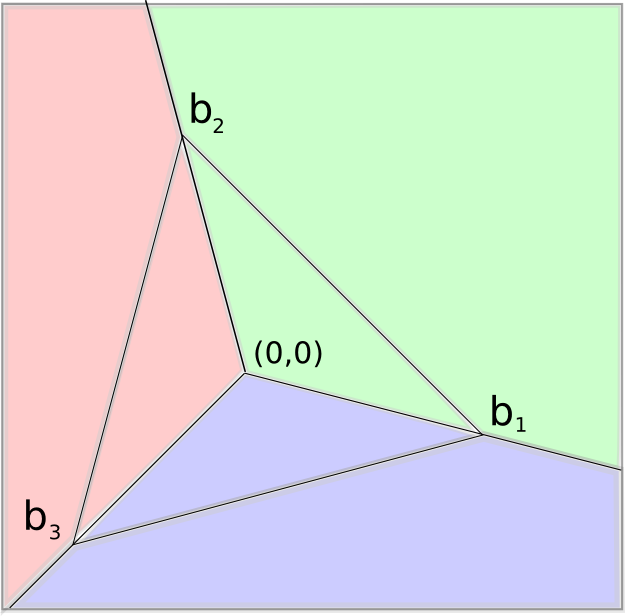
\includegraphics[width=\textwidth]{conesA.png}
%\caption{Illustration of the cone partition. The cones $C_1$, $C_2$, and $C_3$ are denoted with colors red, blue, and green, respectively. }	
%\label{coneA}
%        \end{subfigure}%
%        ~ %add desired spacing between images, e. g. ~, \quad, \qquad etc.
%          %(or a blank line to force the subfigure onto a new line)
%        \begin{subfigure}[b]{0.45\textwidth}
%                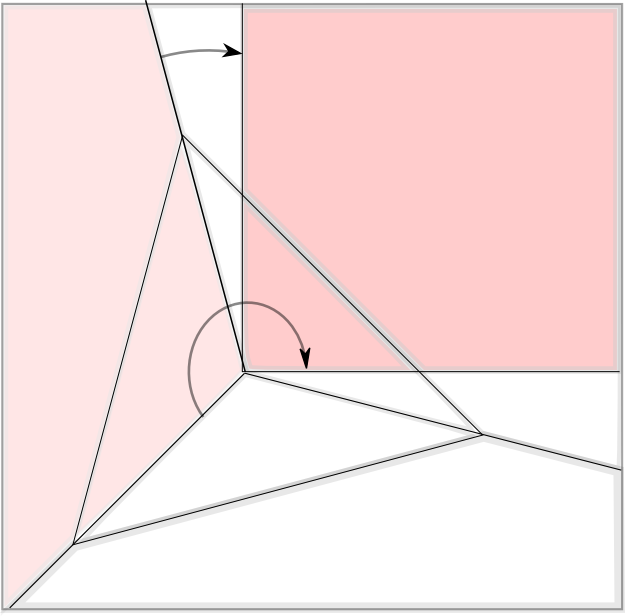
\includegraphics[width=\textwidth]{conesB.png}
%\caption{Illustration of the rotation. In this example $C_1$ is rotated to the convex cone $C_e$ defined by the two standard basis vectors $\boldsymbol{e}_1$ and $\boldsymbol{e}_2$}
%\label{coneB}
%        \end{subfigure}
%        \caption{Illustration of the model when the event can take $K = 3$ different outcomes.}
%\end{figure}
%
%
%This process is linked to the target event by partitioning the $(K-1)$-dimensional space into $K$ cones with apexes at the origin. Denote these cones with $C_k$ for $k = 1, \dots, K$. The target event results in the $k$th outcome if $\boldsymbol{X}_S \in C_k$. Given that the outcomes do not have a particular ordering to them, each cone must have the same shape and neighbor every other cone. This can be achieved with a regular $K$-simplex that has been centered at the origin. More specifically, if $A = \frac{1- \sqrt{K}}{K-1}$ and $B = \frac{1+A}{K}$, the $K$ vertices of the simplex are
%\begin{equation*}
%\begin{array}{lllccr}
%\boldsymbol{b}_1& = &(1-B& -B& \dots& -B)'\\
%\boldsymbol{b}_2& = &(-B& 1-B& \dots& -B)'\\
%&\phantom{.}\vdots&\\
%\boldsymbol{b}_{K-1}& = &(-B& -B& \dots& 1-B)'\\
%\boldsymbol{b}_{K}& = &(A-B& A-B& \dots& A-B )'
%\end{array}
%\end{equation*}
%%http://mathoverflow.net/questions/38724/coordinates-of-vertices-of-regular-simplex
%Then $C_k$ is the convex cone defined by all vertices except the $k$th one. That is, 
%\begin{align*}
%C_k &= \{\boldsymbol{b}_1\theta_1 + \dots + \boldsymbol{b}_{k-1}\theta_{k-1} + \boldsymbol{b}_{k+1}\theta_{k+1} + \boldsymbol{b}_{K}\theta_{K} | \theta_1, \theta_2, \dots, \theta_K \geq 0\} 
%\end{align*}
%Figure \ref{coneA} illustrates the construction of the cones under $K = 3$ different outcomes. The cones $C_1$, $C_2$, and $C_3$ are denoted with colors red, blue, and green, respectively. The aggregate probability for the $k$th outcome is computed by integrating over $C_k$ with respect to (\ref{CondMult}). This integration becomes easier if $C_k$ is first transformed into the convex cone defined by the first $K-1$ standard basis functions. Figure \ref{coneB} illustrates the transformation for $C_1$.  Denote the standard cone with $C_e$ and let 
%\begin{align*}
%T_k &= \left(\begin{matrix} 
%\boldsymbol{b}_1& \dots & \boldsymbol{b}_{k-1} & \boldsymbol{b}_{k+1} & \dots & \boldsymbol{b}_K
% \end{matrix}\right) ^{-1}
%\end{align*}
%represent the transformation matrix for $C_k$. Define the function $F(\boldsymbol{x}_0 | \boldsymbol{\mu}, \Sigma)$ of a random variable $\boldsymbol{x} \sim \mathcal{N}_N(\boldsymbol{\mu}, \Sigma)$ as the probability that all of the components of $\boldsymbol{x}$ are \textit{greater or equal} to the corresponding elements in $\boldsymbol{x}_0$. Then the aggregator is 
%\begin{align}
%\P(\boldsymbol{X}_S \in C_k | \boldsymbol{X}) &= \P(T_k \boldsymbol{X}_S \in C_e | \boldsymbol{X}) \nonumber\\
%&= F(\boldsymbol{0} | T_k\boldsymbol{\bar{\mu}}, T_k' \bar{\Lambda}T_k) \label{MultiAggre}
%\end{align}
%By construction the aggregate probabilities for the $K$ outcomes sum to one. The aggregator (\ref{MultiAggre}) provides the map from a probability forecast to the corresponding probit forecast made by an expert. More specifically, the probability forecasts for the $k$th outcome made by the $j$th expert is
%\begin{align*}
%p_{kj}&= F(\boldsymbol{0} | T_k\boldsymbol{X}_{I_j}, (1-\delta_j)T_k'T_k)
%\end{align*}
%This map establishes $K$ equations with $K$ unknown values. Therefore $\boldsymbol{X}_{I_j}$ can be determined based on the probability forecasts. Similarly to the binary case, the expert's probability forecasts are marginally uniform over the vertices of the $K$-simplex when $\delta_j = 1$. The marginal distribution converges to a point mass at the center of the simplex, i.e. the point $(1/K, 1/K, \dots, 1/K)$ as $\delta_j \to 0$. This ``point of ignorance" has been acknowledged previously in the literature (see, e.g., \cite{fox2003partition, see2006between, satopaa}). 



\section{Discussion}

% What did we learn from this ?

% 1. In the real world there does not seem to be the two sources of reverse-extremization. X
% 2. Illustrated that parameters can be estimated X
% 2b. Future work: learning about overlap structures X
% 3. Summarize main observations: 
% (i) extremization increases as a function of information in the group. X
% (ii) Voting works well under high diversity. 
% 4. Process can be repeated for something else besides extremization X
% 5. Limitation: Discuss optimality constraint 
% 6. The model checks with intuition. X

% 7. Overall, the procedure resembles voting. Therefore voting can be expected to work well in practice when the voters form a very knowledgable and diverse group of experts.

This paper began by introducing a partial information model for probability forecasts. The model was used to derive and study an entire class of probability aggregators that are closely linked to the actual environment of probability forecasts. As a result, many of the results aligned well with intuition.  In particular, the analysis showed that the amount of extremizing is positively associated with the total amount of information in the group of experts, and also presented two main sources of reverse-extremization: i) a dominant expert whose information forms (or at least approximates) a superset of information, and ii) highly influential information that ultimately decides the outcome of the target event. Given that many previous studies have found extremization to improve aggregate predictions in the real world, it is likely that these sources are not very common in practice. 

These sources were central in guiding the discussion towards the non-overlapping and compound symmetric information structures. Given that the latter is unaffected by both sources of reverse-extremization, the corresponding aggregator always extremizes. Therefore it is suitable for aggregation of expert beliefs in the absence of a separate training set. It is important to emphasize that the means of arriving at this aggregator are not restricted to the study of extremization. Therefore, if in the future some other characteristic is found to be important in probability forecasting, it is possible to use the partial information model to perform a case-by-case analysis, understand the main driving factors of this characteristic, and then develop novel methodology with the desired properties. 


New aggregators can also be developed by finding new ways to estimate the information structure. It seems difficult, if possible at all, to estimate the information structure in its full generality. Therefore it will be necessary to pose some constraints on the structure. Section \ref{compound} illustrated this by giving explicit instructions on how to estimate the structure under compound symmetric information. Unfortunately, this structure has poor limiting behavior. Part of our future work is to develop a class of information structures that is  both estimable and realistic for large number of experts.  A different alternative is to construct a realistic prior distribution for the information structure, update this prior to a posterior distribution via the multivariate normal likelihood function, and then marginalize the information structure with respect to its posterior distribution.  

 
 Other future directions could  remove some of the obvious limitations of the model. For instance, assuming that the experts' produce optimal probability forecasts given their private information sets may not be a realistic assumption. The experts may believe in false information, hide their true beliefs, or be biased for many other reasons. This could be expressed in the model by introducing an error term, possibly with a mean of zero, that is added to the experts' optimal forecasts. Even though adding such an error term might improve the real-world performance of resulting aggregators, it is hardly necessary in this paper as the results are conceptual. After all, the cleanest discussion follows from assuming optimal forecasts. This assumption is natural if a subjective probability is considered logical and objectively determined by evidence (see, e.g., \cite{carnap1962logical, jeffreys1998theory, keynes2004treatise}). \cite{dawid1995coherent} also argue that an aggregator should be hesitant in involving experts' whose world views differ radically from that of the decision maker. 
 
% They state that ``[a]t any rate, the condition has sufficient \textit{prima facie} appeal to make it worthwhile to investigate its consequences."

 
 
 


%\bibliographystyle{plain}
\bibliographystyle{plainnat}
\bibliography{biblio}		% expects file "myrefs.bib"



\end{document}
